\documentclass[a4paper,oneside]{report}
\usepackage{color}              %Farben, f.r \definecolor{}
\usepackage{amssymb}            %Mathematische Symbole
\usepackage{amsthm}             %Besseres \newtheorem
\usepackage{amsmath}            %Mathematische Umgebungen
\usepackage{mathtools}          %\xRightarrow, etc
\usepackage{mathrsfs}           %enthaelt \mathscr
\usepackage{graphicx}
\usepackage{enumerate}          % in-place numerations def.
\usepackage{fullpage}
\usepackage{array}
%\usepackage{multicol}
%\usepackage[notref,notcite]{showkeys}
%\usepackage{algorithm,algorithmic}
\usepackage{color}
\usepackage{graphicx}
\usepackage{xypic}
\entrymodifiers={+!!<0pt,\fontdimen22\textfont2>}
\usepackage[all]{xy}

%-----------------------------
%Hugrún's additions
\usepackage{hyperref}
\usepackage{blkarray}

\usepackage{tikz}
\newcommand{\LD}{\langle}
\newcommand{\RD}{\rangle}
\usepackage{tikz}
\usepackage{tikz,fullpage}
\usetikzlibrary{arrows,%
                petri,%
                topaths}%
\usepackage{tkz-berge}
\usepackage[position=top]{subfig}

%------------------------

\newtheoremstyle{myremark} % name
    {7pt}                    % Space above
    {7pt}                    % Space below
    {}  	                 % Body font
    {}                           % Indent amount
    {\bf}       	         % Theorem head font
    {.}                          % Punctuation after theorem head
    {.5em}                       % Space after theorem head
    {}  % Theorem head spec (can be left empty, meaning ‘normal’)

\theoremstyle{plain}
\newtheorem{lemma}{Lemma}[chapter]
\newtheorem{theorem}[lemma]{Theorem}
\newtheorem{fact}[lemma]{Fact}
\newtheorem{definition}[lemma]{Definition}
\newtheorem{corollary}[lemma]{Corollary}
\newtheorem{proposition}[lemma]{Proposition}
\newtheorem{conjecture}[lemma]{Conjecture}
\newtheorem{observation}[lemma]{Observation}
\newtheorem{problem}[lemma]{Problem}
\newtheorem{notation}[lemma]{Notation}
\newtheorem*{claim}{Claim}

\theoremstyle{myremark}
\newtheorem{remark}[lemma]{Remark}
\newtheorem{example}[lemma]{Example}

%-------------------------
% OUR MACROS
\newcommand{\compl}[1]{\overline{#1}}
\newcommand{\real}{\mathbb{R}}
\newcommand{\RR}{\real}
\newcommand{\ZZ}{\mathbb{Z}}
\newcommand{\vol}{\mathrm{vol}}
\newcommand{\oo}[1]{\overline{#1}}

%------------------------

\title{\bf Graph coloring}
\author{Micha{\l} Adamaszek \and ? \and ?}
%------------------------
\begin{document}

\maketitle
\tableofcontents

\chapter{Preface}

These lecture notes come from a master-level course \emph{Graph coloring}, taught by the first author at the Department of Mathematical Sciences of the University of Copenhagen in spring 2016.

\medskip
Despite the name, this is not what one would call a comprehensive course in graph coloring. Instead, graph coloring problems serve only as a convenient excuse to familiarize the students, who may never have taken a more advanced combinatorics course, with interesting combinatorial techniques. The purpose is rather to give a taste of tools from linear algebra, calculus, combinatorics and geometry and demonstrate a few classical combinatorial theorems and their applications. It also has a bit of an experimental flavour and includes short programming exercises in Sage.

\medskip
Each chapter ends with a series of exercises, preferably to be solved with the guidance of an instructor. The last chapter contains exam problems with short hints. This division does not imply a gradation of difficulty --- some of the chapter exercises are quite challenging!

\medskip
We are grateful for the contribution by the students who took notes during the course: Giorgia Laura Cassis, Hugr\'un Fj\'ola Hafsteinsd\'ottir, Rolf J{\o}rgensen, Mathis Elmgaard Isaksen, Sokratis Theodoridis, Mortan Janusarson Thomsen, Kristoffer Holm Nielsen. Most of these notes are based on their writeup.

\medskip
The LaTeX source of these lecture notes is available under the GNU GPL license from \url{http://github.com/aszek/chromatic}. 
\chapter{Temporary}

\section{Notation}

A graph is $G=(V,E)$ and it has $n=|V|$, $m=|E|$. If there are more graphs the next one is $H$. A coloring with $c$ colors is a function $f:V\to \{1,\ldots,c\}=C$. The chromatic number is $\chi$. A bipartite graph has parts $A,B$, or $X,Y$.


\section{Aha foo bar}
This is just a testing ground for now.

Here is ade finition

\begin{definition} We say that a \emph{definition} is a definition is
\begin{equation}
\label{eq:def-eq-temp}
\int_M d\omega = \int_{\partial M} \omega
\end{equation}
\end{definition}

On the other hand, here is a remark:

\begin{remark}
I would like the contents of a remark not to be italicised.
\end{remark}

\section{Section}
It would be good to split each chapter into 2-4 sections.

\section{Including sage code}
We include SAGE source code like this:

\begin{verbatim}
def FunnyGraph(n):
    c = graphs.CompleteGraph(n)
    c.delete_edges(graphs.CycleGraph(n).edges())
    return graphs.MycielskiStep(c).join(graphs.WheelGraph(n+1))

G = FunnyGraph(99)
\end{verbatim}

At the very end I will implement it using a pygmentize highlighter for python.

Figures can be drawn in tikz or whatever, or included from another file. In any case, it would be good to have every figure inside a figure environment with a label and caption.

\section{TODOs}
List of todos for MA:
\begin{itemize}
\item Remove this file
\item Add pygmentize
\item Expand and check bibliography
\end{itemize}


\section{Notation}
(This section is not temporary. In fact, it will become this whole chapter.)

\begin{center}
\begin{tabular}{ll}
$G, H, \ldots$          	&  graphs \\
$G=(V,E)$					&  vertices and edges of a graph \\
$\compl{G}$					&  graph complement \\
$L(G)$						&  line graph of $G$ \\
$G\setminus e$				&  edge removal \\
$G/e$						&  edge contraction \\
$K_n$						&  $n$-vertex complete graph \\
$K_{n,m}$					&  complete bipartite graph \\
$C_n$						&  $n$-vertex cycle \\
$P_n$						&  $n$-vertex path \\
$Q_d$						&  the $d$-dimensional cube graph \\
$M(G)$						&  the Mycielski construction on $G$ \\
$\Delta(G)$					&  maximal vertex degree in $G$ \\
$\delta(G)$					&  minimal vertex degree in $G$ \\
$\omega(G)$					&  clique number \\
$\alpha(G)$					&  independence number \\
$\chi(G)$					&  chromatic number \\
$\chi_l(G)$					&  list chromatic number \\
$\chi'(G)$					&  edge chromatic number \\
$P_G(t), P(G,t)$			&  chromatic polynomial \\
$G(n,p)$					&  random graph $G(n,p)$ \\
$G+H$						&  join of graphs \\
$G\sqcup H$					&  disjoint union of graphs \\
$\real, \ZZ$					& real numbers, integers
\end{tabular}
\end{center}

\chapter{Basic graph theory}

Graph theory as we know it begins with the problem of \textit{Seven Bridges of K\"onigsberg} (now Kaliningrad, Russia), solved by Euler 1736. The problem asks if one can take a our of the city (see map) passing through each bridge exactly once? The answer is (of course) \emph{no}: the reason is that the graph representing the problem has $4$ vertices of odd degree, whereas the existence of said tour imples there can be at most two of those. See if you can turn this into a proof by the end of the chapter.

\section{Introduction}

The purpose of this chapter is to introduce and standardize basic notions and language of graph theory and make sure everyone is on the same page. In this course we mainly study simple graphs:

\begin{definition}
A \emph{simple, undirected graph} is a pair $G=(V,E)$ where $V$ is the set of \emph{vertices} and 
$E \subseteq {V\choose 2}$, is the set of \emph{edges}. 
\end{definition}

We will be using the following notation, sometimes dropping part of the decorations when it is clear what object is referred to:

\begin{itemize}
    \item $xy\in E(G)$ for $\{x,y\}\in E(G)$,
    \item $N_G(x)=\{y: xy\in E(G)\}$ is the \emph{neighborhood} of $x$ in $G$.,
    \item if $xy\in E(G)$ we say $x,y$ are \emph{adjacent} or \emph{neigbors} in G,
    \item a vertex is \emph{incident} to the edges that contain it,
\end{itemize}

Unless otherwise noted, the word \textbf{graph} always denotes an \textbf{undirected, simple} and \textbf{finite} graph.

Other types of graphs appear in the literature and we may use them sporadically. They are, for example:

\begin{itemize}
    \item A multi-graph (multiple edges between a specific pair of vertices).
    \item A directed graph (the edges have a direction, i.e. $E\subseteq V\times V$).
    \item A graph with loops (possible edge from a vertex to itself).
    \item A labelled graph (a labelled version of any other graph type where the edges carry some more information).
\end{itemize}


\begin{example}
Some key examples of families of graphs.
\begin{itemize}
    \item \emph{Cycles:} $C_n,\ n\geq 3$.\newline
    $V=\{1,\dots,n\}$\newline
    $E=\{12,23,\dots,(n-1)n,n1\}$
    \item \emph{Paths:} A subset of a cycle, $P_n,\ n\geq 1$
    \item \emph{Complete graphs:} $K_n,\ n\geq 1$\newline 
    $V=\{1,\dots,n\}$\newline
    $E={V \choose 2}$, all possible pairs of $V$\newline
    Note! $|E(K_n)|={n \choose 2}=\frac{n(n-1)}{2}$
    \item $\overline{K_n},\ n\geq 1$ (the complement of a complete graph)\newline 
    $V=\{1,\dots,n\}$\newline
    $E=\varnothing$
    \item \emph{The Empty Graph:} denoted $\varnothing$;\newline 
    $V(\varnothing)=\varnothing$\newline
    $E(\varnothing)=\varnothing$
\end{itemize}
\end{example}

\begin{definition}
The complement of $G$ is the graph $\overline{G}$ such that
$$
V(\overline{G})=V(G),\quad E(\overline{G})= {V(G)\choose 2}\setminus E(G)
$$
\end{definition}

\begin{example}
$Q_n,\ n\geq 1$\newline
$V(Q_n)=\{(x_1,\dots,x_n):\ x_i\in\{0,1\}\}$, all binary sequences of length $n$.\newline
$(x_1,\dots x_n)(y_1,\dots,y_n)\in E(Q_n)$ iff $(x_1,\dots x_n)(y_1,\dots,y_n)$ are different in exactly one position.\newline
\begin{itemize}
    \item $n=1$\newline
    $V(Q_1)=\{0,1\}$\newline
    $E(Q_1)=\{01\}$
    \item $n=2$\newline
    $V(Q_2)=\{00,01,10,11\}$\newline
    $E(Q_2)=\{\{00,10\},\{00,01\},\{01,11\},\{10,11\}\}$
    \item $n=3$\newline
    $V(Q_3)=\{000,001,010,100,011,101,110,111\}$\newline
    $E(Q_3)=\{\{000,001\},\{000,010\},\dots,\{011,111\}\}$
\end{itemize}
\end{example}

\begin{definition}
$G=(V,E)$. For a vertex $v\in V$, the \emph{degree} of $v$, denoted $\deg(v)$, is the number of edges incident to $v$. In other words $\deg(v)=|N(v)|$. A vertex $v$ is called \emph{isolated} if $\deg(v)=0$ and \emph{a leaf} if $\deg(v)=1$.
\end{definition}

\begin{lemma}
$$
\sum_{v\in V(G)} \deg(v)=2\cdot|E(G)|
$$
\end{lemma}
\begin{proof}
This is clear, because the sum counts every edge twice. However, once in a while we can prove something with excessive formalism. For this, let $M$ be a matrix of size $|V|\times |E|$ defined by
\[
    M_{v,e}= 
\begin{cases}
    1,  & \text{if $v$ is incident to $e$}\\
    0,  & \text{otherwise}
\end{cases}
\]
It is called the \emph{incidence matrix} of $G$.

\begin{example}
$V=\{a,b,c,d\}$ and $E=\{ab,bc,cd\}$.
\[
M=
\begin{blockarray}{cccc}
 & ab & bc & cd \\
\begin{block}{c(ccc)}
  a & 1 & 0 & 0\\
  b & 1 & 1 & 0\\
  c & 0 & 1 & 1\\
  d & 0 & 0 & 1\\
\end{block}
\end{blockarray}
 \]
\end{example}

To continue the proof, note that we can count the number of $1's$ in $M$ in two different ways:
\[
\begin{cases}
    2\times |E|,  & \text{(two $1's$ in each column)}\\
    \sum_{v}^{} \deg(v),  & \text{($\deg(v)\, 1's$ in $n$-th row)}
\end{cases}
\]
What we did is a formal proof using \emph{double counting}.
\end{proof}

\begin{corollary}
The number of vertices of odd degree in every graph is even.
\end{corollary}

Some notions related to vertex degrees deserve their own name.

\begin{itemize}
        \item $\Delta (G)$ is the maximum vertex degree in $G$.
        \item $\delta (G)$ is the minimal vertex degree in $G$.
        \item $G$ is called $d$-regular if all vertices have degree $d$, or equivalently if $\Delta(G)=\delta(G)=d$. (Example: $Q_n$ is $n$-regular)
\end{itemize}

\begin{definition}
A graph $H$ is a called a \emph{subgraph} of $G$ if $V(H)\subseteq V(G)$ and $E(H)\subseteq E(G) $. A subgraph $H$ is called \emph{induced} (by a vertex set $W$) if $V(H)=W$ and $E(G[W])=\{xy; xy\in E(G), x,y\in W\}$.
\end{definition}

We write $H=G[W]$ for the subgraph of $G$ induced by $W\subseteq V(G)$.

\begin{definition}
$f:G\rightarrow H$ is a \emph{graph homomorphism} if $f:V(G)\rightarrow V(H)$, \newline s.t. $xy\in E(G)\Rightarrow f(x)f(y)\in E(H)$
\end{definition}

\begin{lemma}
$1_G:G\rightarrow G$ is homomorphism. $f:G\rightarrow H$, $g:H\rightarrow K$ are homomorphisms, then so is $gf:G\rightarrow K$.
\end{lemma}

\begin{definition}
$G$ and $H$ are \emph{isomorphic} if $\exists\,f:G\rightarrow H$ and $g:H\rightarrow G$ s.t. $gf=1_G, fg=1_H$.
\end{definition}

Deciding if two graphs are isomorphic is computationally hard. Proving non-isomorphism is usually about finding some invariant that distinguishes the two graphs.


\section{Walks, cycles and connectedness}

\begin{definition}
A \emph{walk} in $G$ from $u$ to $v$ ($u,v, \in V(G)$) is a sequence
$$u=x_1,x_2,\dots,x_k=v,$$
such that $x_ix_{i+1} \in E(G)$ for all $i$. This walk is called closed if $u=v$. Moreover:
\begin{enumerate}
\item $G$ s called \emph{connected} if there is a walk between any two vertices,
\item $G$ is called \emph{disconnected} otherwise.
\end{enumerate}
\end{definition}

\begin{definition} The \emph{distance} between $u$ and $v$ ($u,v, \in V(G)$) is
$$d(u,v):=
\begin{cases} 
\text{length of the shortest walk from $u$ to $v$}, & \text{if $\exists$ a walk between $u$ and $v$}\\ 
\infty, & \text{if $\nexists$ a walk between $u$ and $v$}\\
0, & \text{if } u=v
\end{cases}.$$
Moreover the \emph{diameter} of $G$ is
$$diam(G):= \max_{u,v\in V(G)}(d(u,v)).$$
\end{definition}


\begin{lemma} $G$ is disconnected $\Longleftrightarrow \exists$ non-empty sets $X,Y$ with $V(G)=X \cup Y$, $X \cap Y=\emptyset$ such that there is no edge from $X$ to $Y$.
\end{lemma}

\begin{proof}
\emph{$(\Leftarrow)$} Take $u\in X$ and $v \in Y$, then clearly $d(u,v)=\infty$ and $G$ is disconnected.
\\ \emph{$(\Rightarrow)$} If $G$ is disconnected, then we can find $u,v\in V(G)$ with $d(u,v)=\infty$. We define
$$X:=\{x\in V(G): \ d(u,x)<\infty \},$$
$$Y:=V(G) \backslash X.$$
Since $u\in X$ and $v\in Y$, these two sets are non-empty. Moreover there is no edge between these two sets: assume there exist $w\in X,\ z\in Y$ such that $wz \in E(G)$, then $d(u,z)\leqslant d(u,w)+1 <\infty$, which is a contradiction.

(FIGURE)
\end{proof}

\section{Trees and bipartite graphs}

\begin{definition} A \emph{tree} is a connected graph without cycles. A \emph{forest} is a graph, whose every connected component is a tree.
(FIGURE)
\end{definition}

\begin{theorem} The following are equivalent:
\begin{enumerate}
\item $G$ is a tree,
\item $G$ is connected and $|E(G)|=|V(G)|-1$,
\item Every two vertices of $G$ are connected by exactly one path.
\end{enumerate}
\end{theorem}

\begin{proof}
\emph{$(3\Rightarrow 1)$} $G$ is already connected by assumption, hence we must only show that $G$ has no cycles. Assume that we an find one, then all vertices $u,v$ from that cycle are connected by $\geqslant 2$ paths, which is a contradiction.
\\ \emph{$(1\Rightarrow 2)$} We work with induction on the number of vertices (let $|V(G)|=n$). For $n=1$ we clearly have no edges. Assume $n\geqslant 2$. Since $G$ is connected we can choose an edge $e\in E(G)$. Let us take a look at $G-e$ ($G$ without $e$):

(FIGURE)


Removing an edge generates at most $2$ connected components (call them $G_1$ and $G_2$), both without cycles. Since $G$ was a tree, $G_1$ and $G_2$ are connected and $G-e$ is a forest with two components. We can compute
\begin{align*}
|E(G)|&=1+|E(G_1)|+|E(G_2)|\overbrace{=}^{\text{i.a.}}1+|V(G_1)|-1+|V(G_2)|-1=\\
&=|V(G_1)|+|V(G_2)|-1 = |V(G)|-1.
\end{align*}

\emph{$(2\Rightarrow 3)$} Assume we already proved Lemma \ref{Lemma 7}, then we can find a leaf $v\in V(G)$. Let $w$ be the only neighbour of $v$. $G-v$ is again connected and we have
$$|E(G-v)|=|V(G-v)|-1.$$
Working with induction (whose initial step is obvious) we can say that every two vertices in $G-v$ are connected by exactly one path, hence there is also a unique path $x,w,v$ for every $x\in V(G-v)$.
\end{proof}

\begin{lemma} \label{Lemma 7}
Any tree has at least $2$ leaves, provided that it has at least $2$ vertices.
\end{lemma}

\begin{proof}
Let $G$ be a tree with $n$ vertices and $n-1$ edges. Since $G$ is connected, then 
$$\forall v\in V(G): \ deg(v)\geqslant 1.$$
Suppose that we only have $1$ leaf, then
$$\underbrace{2(n-1)}_{\substack{\text{all other vertices}\\ \text{have degree} \geqslant 2}} +\underbrace{1}_{\text{leaf}} \leqslant \sum_{v\in V(G)}deg(v)=2(n-1),$$
which is a contradiction. The same follows if we allow no leaves.
\end{proof}


\begin{definition} $G$ is \emph{bipartite} if there are two sets $A$ and $B$ with $V(G)=A\cup B$, $A\cap B=\emptyset$ such that every edge of $G$ has one end in each part.
\end{definition}

\begin{example} We can use bipartite graph to illustrate a scheduling problem.
(FIGURE)
\end{example}

\begin{example}
\begin{itemize}
\item Complete bipartite graphs ($K_{n,m}$): two sets $A$ and $B$ (with $|A|=n$ and $|B|=m$) with all the possible edges in between.
\item Trees are bipartite. 
\item $n$-cubes graphs ($Q_n$): $V_n:=\{(x_1,\dots,x_n): \ x_i \in \{0,1\}\}$ and then define 
$$A_n:=\{(x_1,\dots,x_n) \in V_n: 2 \mid \sum_{i=1}^n x_i\},$$
$$B_n:=\{(x_1,\dots,x_n) \in V_n: 2 \not| \ \sum_{i=1}^n x_i\}.$$
Moving on one edge clearly changes the parity of the sequence, hence $V_n=A_n\cup B_n$ defines a bipartite graph.
\item Cycles: $C_{2n}$ is bipartite, $C_{2n+1}$ is not bipartite (for $n\in \mathbb{N}$).
\end{itemize}
\end{example}

\begin{theorem} \emph{(K\"{o}nig)}
$G$ is bipartite iff there is no closed walk of odd length.
\end{theorem}

\begin{proof}
\emph{$(\Leftarrow)$} If we start in $A$, after an odd number of steps we will be in $B$ (since each step brings to the other side of the graph).
\\ \emph{$(\Rightarrow)$} Assume that $G$ is connected (if not, work separately in each connected component). Pick $v\in V(G)$ and define
$$A:=\{w\in V(G): \exists \text{ an even-length walk } v\rightarrow w\},$$
$$B:=\{w\in V(G): \exists \text{ an odd-length walk } v\rightarrow w\}.$$
\begin{itemize}
\item $A\cup B=V(G)$, since $G$ is connected.
\item $A\cap B=\emptyset$, since otherwise we could find the following situation for a $w\in A\cap B$:

(FIGURE)

This means we would have an odd closed walk.
\item There is no edge between two vertices in $A$ (resp. $B$), otherwise we would have the following situation:

(FIGURE)

\end{itemize}
\end{proof}

\section{Cliques and independent sets}
\begin{definition}
\begin{itemize}
\item $W\subseteq V(G)$ is a \emph{clique} if for all $x,y\in W$, $x\neq y$, we have $xy\in E(G)$,
\item $W\subseteq V(G)$ is an \emph{independent set} if for all $x,y\in W, \ xy\notin E(G)$.
\end{itemize}
\end{definition}

\begin{remark} A clique is a subgraph that is a complete graph.
\end{remark}

\begin{example} The followings are examples of cliques.
(FIGURE)
\end{example}

\begin{example} The followings are examples of independent sets.
(FIGURE)
\end{example}

\begin{definition}
\begin{itemize}
\item The \emph{clique number} of $G$, $\omega(G)$, is the cardinality of the biggest clique in $G$,
\item The \emph{independence number} of $G$, $\alpha(G)$, is the cardinality of the biggest independent set in $G$.
\end{itemize}
\end{definition}

\begin{observation}
\begin{enumerate}
\item $\alpha(G)=\omega(\overline{G})$.
\begin{proof}
A clique in $G$ is an independent set in $\overline{G}$ and vice versa.
\end{proof}
\item If $G$ is bipartite, then $\omega(G)\leqslant 2$.
\begin{proof}
If there is a triangle, then two of the vertices have to be in the same part of the bipartite graph, which is impossible by definition.
\end{proof}
\item $\omega(G)\leqslant 2$ does not imply that $G$ is bipartite.
\begin{proof}
$C_5$ (which is not bipartite since it is an odd cycle) has $\omega(C_5)=2$.
\end{proof}
\end{enumerate}
\end{observation}

\begin{definition} Graphs with $\omega(G)\leqslant 2$ are usually called triangle-free.
\end{definition}

\begin{example}
\begin{itemize}
\item $\omega(C_n)=
\begin{cases} 
3, & \text{if } n=3\\ 
2, & \text{if } n\geqslant 4
\end{cases}.$
\item $\alpha(C_n)=
\begin{cases} 
\frac{n}{2}, & \text{if } 2\mid n\\ 
\frac{n-1}{2}, & \text{if } 2\not| \ n
\end{cases}.$
\item $G$ bipartite (i.e. $V(G)=A\cup B$), then $\alpha(G)\geqslant max\{|A|,|B|\}$.
\item $\omega(K_n)=n$ and $\alpha(K_n)=1$.
\end{itemize}
\end{example}

\begin{remark} $\alpha$ and $\omega$ are hard (meaning $NP$-hard) to compute.
\end{remark}

\begin{lemma}
$\alpha(G)\geqslant \frac{|V(G)|}{1+\Delta(G)}$.
\end{lemma}

\begin{proof} We must find an independent set of size at least $\frac{|V(G)|}{1+\Delta(G)}$ and we will work by induction in order to do that. Take an arbitrary vertex $v\in V(G)$ and consider the graph 
$$G':=G-v-N_G(V).$$
Clearly $\Delta(G')\leqslant \Delta(G)$. Using the induction assumption, $G'$ has an independent set $X$ of size at least
$$\frac{|V(G')|}{1+\Delta(G')}.$$
Consider $X\cup \{v\}$, which (by construction) is an independent set in $G$.
$$|X\cup \{v\}|=|X|+1\geqslant\frac{|V(G')|}{1+\Delta(G')}+1\geqslant \frac{|V(G)|-(1+\Delta(G))}{1+\Delta(G)}+1=\frac{|V(G)|}{1+\Delta(G)},$$
thanks to $\Delta(G')\leqslant \Delta(G)$ and considering that $1+\Delta(G)$ is the biggest number of vertices we can take away while defining $G'$.
\end{proof}

(The greedy algorithm) The following loop iterates $\geqslant \frac{|V(G)|}{1+\Delta(G)}$ times.
\begin{enumerate}
\item Take $v\in V(G)$,
\item Remove $v$ and $N_G(v)$ (at most $1+\Delta(G)$ vertices),
\item Iterate using $G':=G-v-N_G(V)$.
\end{enumerate}

\begin{lemma} If $f:G\longrightarrow H$ is a graph homomorphism, then $f^{-1}(v)$ is an independent set for all $v\in V(H)$.
\end{lemma}

\begin{proof}
Suppose that $x,y\in f^{-1}(v)$ and $xy\in E(G)$. Then, since $f$ is a graph homomorphism, we would have $f(x)f(y)\in E(H)$, which is impossible since $f(x)=f(y)=v$.
\end{proof}




\section{Exercises}

\begin{enumerate}
\item Show that in the definition of connectedness and distance we can replace \emph{walk} with \emph{path}, and that in K\"onig's theorem we can replace \emph{closed walk} with \emph{cycle} (and even \emph{induced cycle}).

\item Prove that every graph has two vertices of the same degree.
\item In a class with $19$ students each person sends a Valentine's Day card to exactly three other students. Is it possible that each student receives cards from the same three students to whom he/she sent cards?
\item Draw all isomorphism classes of trees on $n=1,2,3,4,5$ vertices.
\item What is the maximal possible number of edges in a disconnected graph on $n$ vertices?
\item Let $G$ be a graph with minimum vertex degree $d\geq 2$. Prove that $G$ contains a cycle of length at least $d+1$.
\item Prove that if $G$ is disconnected then its complement $\overline{G}$ is connected.
\item Classify all connected $2$-regular graphs.
\item Find $\alpha(Q_k)$.
\item For which $n$ is there a homomorphism $C_n\to K_2$\ ?
\item For which $n,m$ is there a homomorphism $C_n\to C_m$\ ?
\end{enumerate}
\chapter{Vertex coloring}

\section{Definitions and examples}

Goal: Assign colours to the vertices of a graph, such that adjacent vertices have different colours (the problem is optimized by finding the minimal number of colours needed for this process).

\begin{example}
\begin{enumerate}
\item Colouring a land-map, such that the countries that share a border have different colours. In this case the vertices represent the countries and we draw an edge whenever two countries share a border.
\item Scheduling the timetable for an exam session. In this case the vertices represent the different subjects offered and we draw an edge whenever there is at least a student following both courses. Minimizing the number of colours means programming the minimal number of exam-spots, such that each student can take all the exams he/she applied for.
\end{enumerate}
\end{example}

\begin{example} Take a graph $G$ with $81$ vertices forming a $9\times9$ grid, such that the following conditions are satisfied:
\begin{itemize}
\item Every row is a clique,
\item Every column is a clique,
\item If we divide the grid forming $9$ $3\times 3$ subgrids, each of these is a clique.
\end{itemize}
Then each possible colouring represents the solutions of a Sudoku.
\end{example}

\begin{definition} A \emph{(vertex-)colouring} of $G$ with colour set $C$ is a function
$$c:V(G)\longrightarrow C,$$
such that if $xy\in E(G)$, then $c(x)\neq c(y)$.
\end{definition}

\begin{definition} The \emph{chromatic number} $\chi(G)$ is the smallest number $k$ for which there is a colouring of $G$ with $k$ colours. If $\chi(G)\leqslant k$, then $G$ is called \emph{$k$-colourable}.
\end{definition}

\begin{definition} Each $c^{-1}(i)$ is called a \emph{color class}.
\end{definition}

\begin{example}
\begin{itemize}
\item $\chi(P_n)=2$,
\item $\chi(C_n)=
\begin{cases} 
2, & \text{if } 2\mid n\\ 
3, & \text{if } 2\not| \ n
\end{cases},$
\item $\chi(K_n)=n$,
\item $\chi(Q_n)=2$, since $Q_n$ is bipartite. Moreover, $\chi$ of every bipartite graph with at least one edge is $2$.
\end{itemize}
\end{example}

\begin{lemma}
\begin{enumerate}
\item $\chi(G)\leqslant |V(G)|$,
\item $\chi(G)=|V(G)| \Longleftrightarrow G$ is complete,
\item $\chi(G)=1 \Longleftrightarrow G \simeq \overline{K_n},$
\item $\chi(G)=2 \Longleftrightarrow G$ is bipartite and has at least one edge.
\end{enumerate}
\end{lemma}

\begin{proof}
\begin{enumerate}
\item $c: |V(G)| \longrightarrow  |V(G)|$ with $c(v)=v$ is a colouring with exactly $|V(G)|$ colours.
\item One direction is obvious. Let us assume $G$ is not complete, then we can find $x,y\in V(G)$ with $xy\notin E(G)$. Set $c(x)=c(y)$ and colour all the other $|V(G)|-2$ vertices with different colours: this is a colouring with $|V(G)|-1$ colours.
\item One direction is obvious. For the other look at $c:V(G)\longrightarrow \{1\}$ with $c(x)=c(y)$ for all $x,y\in V(G)$. This implies $xy\notin E(G)$ for all $x,y\in V(G)$, hence $G \simeq \overline{K_n}$.
\item One direction is obvious. For the other, if $\chi(G)=2$ then it suffices to define $A:=c^{-1}(1)$ and $B:=c^{-1}(2)$ to find the partition of the set $V(G)$.
\end{enumerate}
\end{proof}

\begin{remark}
Already determining whether $\chi(G)\leqslant 3$ or $\chi(G)\geqslant 4$ is hard.
\end{remark}

\begin{observation}
Every color class is an independent set.
\end{observation}
\begin{proof}
If $c(x) = c(y)$ then $xy \notin E(G)$.
\end{proof}

\begin{lemma}
The following are equivalent:
\begin{enumerate}[(1)]
\item $G$ is $k$-colorable
\item $V(G)$ can be partioned into $k$ independent sets
\item There exists a graph homomorphism $G \rightarrow K_k$
\end{enumerate}
\end{lemma}
\begin{proof}
(1) $\Leftrightarrow$ (2): Assume (1) and choose a coloring $c \colon G
\rightarrow \{1,\ldots,k\}$. Then $c^{-1}(1),\ldots,c^{-1}(k)$
partitions $G$ into $k$ independent sets. On the other hand if (2) holds
we can write $V(G) = V_1 \cup \cdots \cup V_k$ where each $V_j$ is an
independet set and $V_i \cap V_j = \emptyset$ when $i \neq j$. Define a
coloring $c \colon G \rightarrow \{1,\ldots,k\}$ by $c(v) = i$ if $v \in
V_i$. Then $c$ is clearly a coloring. So we have that (1)
$\Leftrightarrow$ (2).

(2) $\Leftrightarrow$ (3): If $f \colon G \rightarrow K_k$ is a
homomorphism then $f^{-1}(i)$ is an independent set. This shows (3)
$\Rightarrow$ (2). Suppose $V(G) = V_1 \cup \cdots \cup V_k$, $V_i \cap
V_j = \emptyset$, with each $V_i$ an independent set. Define $f \colon G
\rightarrow K_k$ by $f(v) = i$ if $v \in V_i$. If $vw \in E(G)$ then $v
\in V_i$ and $w \in V_j$ for $i \neq j$. Then $f(v)f(w) = ij \in E(K_k)$
since $i \neq j$.
\end{proof}

The next lemma says that ``bigger graphs have bigger chromatic
numbers''.
\begin{lemma}
If $H \subset G$ ($H$ is a subgraph of $G$) then $\chi(H) \le \chi(G)$.
\end{lemma}
\begin{proof}
Any coloring $c \colon V(G) \rightarrow C$ restricts to a coloring $c
\colon V(H) \rightarrow C$.
\end{proof}


\begin{lemma}
For any graph $G$
\begin{enumerate}[(1)]
\item $\chi(G) \ge \omega(G)$
\item $\chi(G) \ge \frac{|V(G)|}{\alpha(G)}$
\end{enumerate}
\end{lemma}
\begin{proof}
(1): If $\omega(G) = k$, then $G$ contains a clique on $k$ vertices,
i.e. $K_k \subset G$. Then $k = \chi(K_k) \le \chi(G)$ by the lemma.

(2): Suppose $\chi(G) = k$. Then some color class has size at least
$\frac{1}{k}|V(G)|$. Therefore we have an independent set of size $\ge
\frac{1}{k}|V(G)|$, which means $\alpha(G) \ge \frac{1}{k}|V(G)|$.
\end{proof}

\begin{example}
$\chi(C_{2n + 1}) = 3$ although $\omega(C_{2n + 1}) = 2$ for $n \ge 2$.
So it can happen that $\chi > \omega$.
\end{example}

\section{Greedy algorithm(s)}
\begin{definition}
\emph{The greedy coloring} relative to a vertex ordering $v_1, \ldots
v_n$ of the vertices of $G$ is obtained by coloring in this order
subject to the rule:
\[
c(v_i) = \text{ first available color that does not appear among }
N(v_i) \cap \{v_1,\ldots v_{i-1}\}
\]
\end{definition}

\begin{theorem}
The greedy algorithm uses at most $\Delta(G) + 1$ colors. In particular
$\chi(G) \le \Delta(G) + 1$ for any $G$.
\end{theorem}
\begin{proof}
When coloring $v_i$ at most $\Delta(G)$ colors are forbidden, because
$v_i$ has at most $\Delta(G)$ neighbors, so it has $\le \Delta(G)$
already colored neighbors. They use $\le \Delta(G)$ different colors, so
at least one color from $\{1,\ldots,\Delta(G) + 1\}$ is available for
$v_i$.
\end{proof}
\begin{observation}
There is room for improvement if we choose some special vertex ordering.
\end{observation}
\begin{example}
Order the vertices so that $\deg(v_1) \ge \deg(v_2) \ge \cdots \ge
\deg(v_n)$.
\end{example}
\begin{theorem}
With respect to the above ordering, the greedy method uses at most $1 +
\max_i(\min(\deg(v_i),i-1))$ colors. In particular $\chi(G) \le 1 +
\max_i\min(\deg(v_i),i-1)$.
\end{theorem}
\begin{proof}
$v_i$ has at most $\min(\deg(v_i),i-1)$ neighbors among $v_1,\ldots,v_{i-1}$.
\end{proof}


\begin{example}
Order the $v_i's$ so that for each $i$, $v_i$ is some vertex of smallest
degree in $G[\{v_1,\ldots,v_i\}]$ (the sub-graph induced by
$\{v_1,\ldots,v_i\}$).
Construction:
\begin{align*}
v_n &= \text{ vertex of minimal degree in } G \\
v_{n-1} &= \text{ vertex of minimal degree in } G-v_n \\
v_{n-2} &= \text{ vertex of minimal degree in } G-v_n-v_{n-1} \\
\vdots & 
\end{align*}
\end{example}

\begin{theorem}
With this ordering, the greedy method needs at most $1 + \max_H \delta(H)$ colors, 
where the maximum is over all induced subgraphs $H$ of $G$.
\end{theorem}
\begin{proof}
$v_i$ has exactly $\deg_{G[\{v_1,\ldots,v_i\}]}(v_i)$ neighbors among
$v_1,\ldots,v_{i-1}$. But that number is exactly
$\delta(G[\{v_1,\ldots,v_i\}]) \le \max_H \delta(H)$
\end{proof}


\section{Brooks' theorem}

\begin{example}
Where $\chi = \Delta + 1$:
\begin{enumerate}[(1)]
\item $\chi(K_n) = n = \Delta(K_n) + 1$
\item $\chi(C_{2n + 1}) = 3 = \Delta(C_{2n+1}) + 1$
\end{enumerate}
\end{example}

\begin{theorem}[Brooks]
If $G$ is a connected graph, which is not complete, nor an odd cycle,
then $\chi(G) \le \Delta(G)$.
\end{theorem}
\begin{proof}
Let $\Delta = \Delta(G)$. If $\Delta \le 2$ then $G$ is a path or a
cycle, and the result is easy. Assume $\Delta \ge 3$. Pick any vertex $v
\in V(G)$ with $\deg(v) = \Delta$. Let $H = G-v$.  The proof is by
induction on the number of vertices $|V(G)|$. Suppose, for
contradiction, $G$ is not $\Delta$-colorable. $H$ is a graph with
$\Delta(H) \le \Delta$. By induction (since $|V(H)| = |V(G)| - 1$) $H$
is $\Delta(H)$-colorable so in particular $\Delta$-colorable. (Be
careful: what if $H$ is an odd cycle or a complete graph? We dealt with these cases in the exercises). Fix any
coloring $c$ of $H$ with $\Delta$ colors. Since $\deg(v) = \Delta$ we can
assume that all neighbors of $V$ have different colors. Otherwise there is a
spare color we can assign to $v$ and $G$ would be $\Delta$-colorable.
Label the vertices in $N(v)$ such that $N(v) =
\{v_1,\ldots,v_{\Delta}\}$ and $c(v_i) = i$. Define $H_{i,j}$ be the
subgraph of $H$ induced by vertices of colors $i$ and $j$ ($i \neq j$,
$i,j \in \{1,\ldots,\Delta\}$).
\begin{claim}[0]
$H_{i,j}$ is bipartite and $v_i,v_j \in V(H_{i,j})$.
\end{claim}
\begin{proof}
Obvious.
\end{proof}
\begin{claim}[1]
$v_i,v_j$ are in the same connected component $C_{i,j}$ of $H_{i,j}$
\end{claim}
\begin{proof}
If not then $H_{i,j}$ is the disjoint union of two subgraphs: $H_{i,j} =
H_{i,j}^{(1)} \cup H_{i,j}^{(1)}$ such that $v_i \in
H_{i,j}^{(1)}$ and $v_j \in H_{i,j}^{(2)}$. Define a new coloring $c'$ of $H$
by swapping the colors in $H_{i,j}^{(2)}$ i.e. define $c'(v) = i$ if $c(v) = j$
and vice versa for all $v \in H_{i,j}^{(2)}$. (The new $c'$ is still a
coloring). With this new coloring $v_i$ and $v_j$ have the same colors,
so we have a spare color for $v$ which as before is a contradiction.
\end{proof}
\begin{claim}[2]
$C_{i,j}$ is a path.
\end{claim}
\begin{proof}
First note that $\deg_{H_{i,j}}(v_i) = 1$ because otherwise $v_i$ has
two neighbors of color $j$. Moreover $\deg_H(v_i) \le \Delta - 1$. Then
there exist $k \neq i$ such that we can recolor $v_i$ with color $k$ and
still have a coloring of $H$ and we get a spare color for $v$.
Analogously we have $\deg_{H_{i,j}}(v_j) = 1$. Let $u$ be a degree $\ge
3$ vertex in $C_{i,j}$ closest to $v_i$. Then $c(u) = i$ or $c(u) = j$,
assume $c(u) = i$. Again: $\deg_H(u) \le \Delta$, but neighbors of $u$
have at most $\Delta - 2$ colors. We can recolor $u$ with some $k
\neq i,j$. Then $v_i,v_j$ land in different components of $H_{i,j}$
contrary to claim 1. 
\end{proof}
\begin{claim}[3]
$C_{i,j} \cap C_{i,k} = \{v_i\}$ if $i \neq j \neq k \neq i$.
\end{claim}
\begin{proof}
If not then there is some $u \in C_{i,j} \cap C_{i,k}$ such that $u \neq
v_i$. $\deg(u) \le \Delta$ and $u$ has two neighbors of color $j$ and
two of color $k$. Therefore neighbors of $u$ use $\le \Delta - 2$ colors
and we can recolor $u$ with some color $\neq i,j,k$ and get a proper
coloring. The new coloring contradicts claim 1.
\end{proof}
If all of $v_1,\ldots,v_{\Delta}$ are pairwise adjacent then $G =
K_{\Delta + 1}$, or otherwise $\Delta(G) \ge \Delta + 1$.  So, assume without
loss of generality that $v_1v_2 \notin E(G)$. Consider the paths
$C_{1,2},C_{1,3}$. Let $C_{1,2} = v_1u\cdots v_2$. Flip the colors in
$C_{1,3}$. We get a proper coloring of $G$. In this new coloring
$C_{1,2}$ and $C_{3,2}$ both contain $u$ contradicting claim 3.
\end{proof}



\section{Large-$\chi$ triangle-free graphs deterministically and probabilistically}

We know that $\chi(G)\geq\omega(G)$ \\
If $G=C_{2n+1}, \quad n\geq 2$ then $\omega(G)=2,\quad \chi(G)=3$ \\
Q: Is there a graph with $\omega(G)=2$ and $\chi(G)=4$? \\
A: Yes the smallest such is the Gr{\"o}tszch graph on 11 vertices $G_{11}$ \\

It is not possible to bound $\chi(G)$ in terms of $\omega(G)$.
\begin{theorem} 
For any $k\geq2$ there is a triangle-free graph with $\chi(G)=k$
\end{theorem}
\begin{definition}
Suppose $G$ is a graph with $V(G)=\{v_1,..,v_n\}$. The \emph{Mycielski construction} $M(G)$ is a new graph with $V(M(G))=\{v_1 ,..,v_n\}\cup\{u_1,..,u_n\}\cup\{w\}, \quad E(M(G))=\{wu_i,\, i=1,..,n\} \cup \{v_i v_j,\ u_iv_j\ : v_iv_j \in E(G)\}$.

(FIGURE)
\end{definition}

As an example have that $M(K_2)=C_5$ and $M(C_5)=G_{11}$.

\begin{theorem} (restated) If $G$ is triangle-free and $\chi(G)=k$ then $M(G)$ is triangle free and $\chi(M(G))=k+1$.
\end {theorem}
\begin{proof}
\begin{enumerate}
	\item $M(G)$ is still triangle free \\
	The only possibility is a triangle with $1$ vertex from $U$ and 2 vertices from $V$. However, by the definition of $M(G)$ we then have that $v_iv_jv_k$ is a triangle, contradicting that $G$ was triangle-free.
	\item $M(G)$ is $k+1$ colorable \\
	We can color $G$ with $k$ colors (The set $V$ in the picture). We use another color $(k+1)$ for all vertices in $U$, and the last node $w$ is colored with some color different from $(k+1)$ 
	\item $M(G)$ is not $k$-colorable. \\
	Suppose otherwise, $c:V(M(G)) \rightarrow \{1,..,k\}$. Suppose wlog that $w$ has color $k$, then $U$ is colored with $k-1$ colors. (Our goal is to show that we can color $G$ with $k-1$ colors) \\
	Let $A= \{v_i \in V, \, c(v_i)=k\}$. \\
	Recolor $A$ by changing the color of each $v_i$ to $c(u_i)$ \\
	$$
	c'(v_i)=\left\{ \begin{array}{rl}
c(v_i) &\mbox{ if $c(v_i)\neq k$} \\
c(u_i) &\mbox{ if $c(v_i)=k$}
\end{array} \right.
$$
$C'$ uses only colors $ \{1,..,k-1\} $. Let's check that $c'$ is a coloring of $G$. Suppose $c'(v_i)=c'(v_j)$ 
\begin{enumerate}
	\item If both of these $v_i,v_j \notin A$ then $v_iv_j \notin E(G)$  
	\item If $v_i \in A,\, v_j \notin A$. Suppose $v_iv_j \in E(G)$, so that $u_iv_j \in E(M(G))$

(FIGURE)

Then $c(u_i)=c'(v_i)=c'(v_j)=c(v_j)$ Contradicting that $c$ is a coloring of $M(G)$
	\item If $v_i,v_j \in A$. Then $c(v_i)=c(v_j)=k \Rightarrow v_iv_j \notin E(G)$
\end{enumerate}
\end{enumerate}
\end{proof}

Recap: We can have triangle-free graphs with arbitrarily high $\chi$. But is $M(G)$ just a special construction that achieves this? Not really. We will see that in the following:

Goal: Prove that objects with an interesting property $P$ exists by showing that a random object has $P$ with non-zero probability. For example: $P=$"triangle-free and $\chi(G)\geq k$"

\begin{definition} (construction). Fix $V=\{1,..,n\}, \, 0\leq p\leq 1$. Construct a graph on $V$ by taking each edge $ij$, $0 \leq i <j \leq n$ with probability $p$, independently for each each pair. \\
$G(n,p)$ is the probability space of all graphs obtained in this way.

\end{definition}

A graph $G \in G(n,p)$ has probability
$$
\mathbb{P}(G)=p^{|E(G)|}(1-p)^{\binom{n}{2}-|E(G)|}.
$$
The expected number of edges/triangles in a random graph from $G(n,p)$ is
$$
\mathbb{E}[\# \text{edges}]=\binom{n}{2}\mathbb{P}[ij \text{ is an edge}]=p\binom{n}{2}
$$
$$
\mathbb{E}[\# \text{of triangles in } G(n,p)]=\binom{n}{3}\mathbb{P}[ijk \text{ is a triangle}]=\binom{n}{3}p^3
$$
Sage can generate random graphs from $G(n,p)$ (\texttt{graphs.randomGNP(n, p)}). 
For the next part we need a few prerequisites:
\begin{enumerate}
	\item $1-x \leq e^{-x}$,
	\item $\binom{n}{k} \leq n^k$,
	\item Markov's inequality: if $X$ is a non-negative random variable, $t>0$, then $\mathbb{P}[X>t]\leq \frac{1}{t}\mathbb{E}[X]$.
\end{enumerate}
\begin{theorem} For every $k\geq 2$  there is a triangle-free graph with $\chi(G)\geq k$.
\end{theorem}
Remark: Not only "there is" but "there are many".
\begin{proof}
Take $G \in G(n,p)$ where $p=\frac{1}{n^{5/6}}$. Let $X=\#$ of triangles in $G$. \\
$\mathbb{E}[X]=\binom{n}{3}p^3 \leq n^{1/2}$. By Markov's inequality $\mathbb{P}[X>10n^{1/2}]\leq \frac{1}{10}$, which means that a typical $G$ has very few triangles. \\
To show that $\chi(G)$ is "large" we will prove that $\alpha(G)$ is "small". Let $a=\frac{3}{p}\ln{n}$ 
$$
\mathbb{P}[\alpha(G)\geq a] \leq \binom{n}{a}\mathbb{P}[\text{exists independent set of size }a] = \binom{n}{a}(1-p)^{\binom{a}{2}} \leq n^ae^{-p\binom{a}{2}} \rightarrow 0,\quad n\rightarrow \infty
$$
where the last limit can be computed by plugging in the formulae for $p$ and $a$ in terms of $n$.

For sufficiently large $n$ we have $\mathbb{P}[\alpha(G)\geq a]<\frac{1}{10}$. Then $$\mathbb{P}[X<10\sqrt{n} \text{ and } \alpha(G)<a] \geq \frac{8}{10}.$$

We showed, with probability $\geq \frac{8}{10}$, a random graph from $G(n,p), \, p=\frac{1}{n^{5/6}}$, has $<10\sqrt{n}$ triangles, and $\alpha(G)<a<3n^{5/6}\ln{n}$ \\
Completing the proof: \\
Take such a random $G$. Remove at most $10\sqrt{n}$ vertices so we get a triangle free graph $G'$ \\
$|V(G')| \geq \frac{n}{2}$ (for large $n$) and 
$$
\chi(G')\geq \frac{|V(G')|}{\alpha(G')} \geq \frac{n/2}{3n^{5/6}\ln{n}}=\frac{1}{6}\frac{n^{1/6}}{\ln{n}}\rightarrow \infty, \quad n\rightarrow \infty
$$
So $\chi(G')$ can be arbitrarily large
\end{proof}


\section{Basic constructions}
\begin{enumerate}
	\item Disjoint union $G \sqcup H$. $\chi(G \sqcup H)=\max(\chi(G),\chi(H))$. As $G\subseteq G \sqcup H \supseteq H$, we need at least enough colors to color $H,G$ individually.
	\item Wedge $G \vee H$ Graphs joined at a single vertex.

(FIGURE)

$\chi(G\vee H)=\max(\chi(G),\chi(H)$. After coloring $G$ color $H$, perhaps permuting the colors so that they agree on the common vertex..	
	
\item The sum (join) $G+H$. It is the disjoint union together with all edges between $V(G)$ and $V(H)$ \\
$\chi(G+H)=\chi(G)+\chi(H)$. As the colors of $G$ must be different from the colors of $H$.
\item The cartesian product $G \square H$ \\
$V(G \square H) = V(G) \times V(H)$ \\
$\{(u,v),(u',v')\} \text{ is an edge iff } (u=u' \text{ and } vv' \in E(H)) \text{ or } (uu' \in E(G) \text{ and } v=v')$. 

\begin{lemma} $\chi(G \square H)=\max(\chi(G),\chi(H))$
\end{lemma}
\begin{proof}
$G\subseteq G \square H \supseteq H$ so $\chi(G \square H) \geq \max(\chi(G),\chi(H))$. Suppose $G$ and $H$ both have coloring with color set $\{0,..,k-1\}$ ($k=\max(\chi(G), \chi(H))$). Le these colorings be 
$$
f: V(G) \rightarrow \{ 0,..,k-1\},
$$
$$
f': V(H) \rightarrow \{ 0,..,k-1 \}.
$$
Define $F(u,v)=f(u)+f'(v) \mod k$. We will check that $F$ is a coloring. Let $(u,v)(u',v') \in E(G \square H)$. Wlog let $u=u'$ and $vv' \in E(H)$, then:
\begin{align*}
	F(u,v) &=f(u)+f'(v) \mod k \\
	F(u',v') &=f(u')+f'(v') \mod k \\
	         &= f(u)+f'(v') \mod k \\
					&\neq f(u)+f'(v) \mod k  \quad \text{because } vv' \in E(H) \\
					&=F(u,v).
\end{align*}
\end{proof}

\end{enumerate}




\section{Exercises}

\begin{enumerate}
\item Prove that a graph with chromatic number $k$ has at least ${k\choose 2}$ edges.
\item Prove $\chi(G)\leq |V(G)|-\alpha(G)+1$.
\item Suppose we have $n$ straight lines in the plane, no three intersecting at the same point. Let $G$ be the graph whose vertices are the intersection points of the lines, and two of them are adjacent if they appear consecutively on one of the lines. Prove that $G$ is $3$-colorable.
\item Suppose $G$ is $4$-colorable. Prove that $G$ can be written as a union of two bipartite graphs (that means there are subgraphs $H_1,H_2$ of $G$ such that $V(G)=V(H_1)\cup V(H_2)$, $E(G)=E(H_1)\cup E(H_2)$ and $H_1,H_2$ are bipartite).
\item Prove that if $\overline{G}$ is bipartite then $\chi(G)=\omega(G)$.
\item Prove that if an $n$-vertex graph is $k$-colorable then it has at most $\frac{k-1}{2k}n^2$ edges.
\item Show that every graph has a vertex ordering for which the greedy algorithm uses exactly $\chi(G)$ colors.

\item $\max_i\min(\deg(v_i),i-1) \le \Delta(G)$ so this bound is at least as
good as $\Delta(G) + 1$ (often much better).

\item 
A graph is called $k$-critical if $\chi(G)=k$ and $\chi(H)<k$ for every proper subgraph $H\subseteq G$.

\begin{enumerate}
\item Prove that a graph is $3$-critical if and only if it is an odd cycle.
\item Show that a $k$-critical graph $G$ has $\delta(G)\geq k-1$.
\item Suppose $G$ is $k$-critical and $e\in E(G)$. Show that every $(k-1)$-coloring of $G-e$ assigns different colors to the endpoints of $e$.
\item Prove that $C_5+K_k$ is $(3+k)$-critical.
\end{enumerate}

\item Show that $\chi(G)\geq h$ iff $\alpha(G \square K_k) \geq |V(G)|$.
\end{enumerate}
\chapter{Planar graphs}

In this part we are going to focus on one of the most classical (and historical) topics in graph coloring: vertex colorings of planar graphs. 

\begin{definition}
$G$ is \emph{planar} if it can be drawn on ${\rm I\!R^2}$(the plane) so that edges intersect only at their common endpoints.
We call such a drawing an \emph{"embedding"}(some authors say \emph{"drawing"}).
\end{definition}

\begin{example}

\begin {tikzpicture}

\draw   
           node[fill,circle,inner sep=0pt,minimum size=3pt] (n1) at (0,0) {}
	node[fill,circle,inner sep=0pt,minimum size=3pt] (n2) at (1,0) {} 
	node[fill,circle,inner sep=0pt,minimum size=3pt] (n3) at (0,1) {} 
	node[fill,circle,inner sep=0pt,minimum size=3pt] (n4) at (1,1) {}
[line width = 1 pt, black, -] (n1) edge (n4)
[line width = 1 pt, black, -] (n2) edge (n3)
[line width = 1 pt, black, -] (n1) edge (n2)
[line width = 1 pt, black, -] (n2) edge (n4)
[line width = 1 pt, black, -] (n4) edge (n3)
[line width = 1 pt, black, -] (n3) edge (n1)
;
\end{tikzpicture}
       $K_4$ not an embedding
\begin {tikzpicture}
\newcommand*{\OutAngle}{60}
 \newcommand*{\ArcMax}{1.2}
\draw
	node[fill,circle,inner sep=0pt,minimum size=3pt] (n1) at (0,0) {}
	node[fill,circle,inner sep=0pt,minimum size=3pt] (n2) at (1,0) {} 
	node[fill,circle,inner sep=0pt,minimum size=3pt] (n3) at (0,1) {} 
	node[fill,circle,inner sep=0pt,minimum size=3pt] (n4) at (1,1) {}
[line width = 1 pt, black, -] (n1) edge (n2)
[line width = 1 pt, black, -] (n1) edge (n2)
[line width = 1 pt, black, -] (n2) edge (n4)
[line width = 1 pt, black, -] (n4) edge (n3)
[line width = 1 pt, black, -] (n3) edge (n1)
(0, 1) to[out=\OutAngle, in=135]
    (\ArcMax, \ArcMax) to[out=-45, in=90-\OutAngle]
    (1, 0) -- cycle
;
\end{tikzpicture}
embedding ($K_4$ is planar)
\newline
\newline
\begin {tikzpicture}
\draw 
%node[fill,circle,inner sep=0pt,minimum size=3pt] (n1) at (0,0) {}
node[fill,circle,inner sep=0pt,minimum size=3pt] (n2) at (-0.5,0) {}
node[fill,circle,inner sep=0pt,minimum size=3pt] (n3) at (0,0.5) {}
node[fill,circle,inner sep=0pt,minimum size=3pt] (n4) at (0.5,0) {}
node[fill,circle,inner sep=0pt,minimum size=3pt] (n5) at (0,1) {}
[line width = 1 pt, black, -] (n2) edge (n4)
%[line width = 1 pt, black, -] (n1) edge (n4)
[line width = 1 pt, black, -] (n3) edge (n5)
[line width = 1 pt, black, -] (n2) edge (n5)
[line width = 1 pt, black, -] (n4) edge (n5)
[line width = 1 pt, black, -] (n3) edge (n4)
[line width = 1 pt, black, -] (n2) edge (n3)
;
\end{tikzpicture}
straight line-embedding
\end{example}

\begin{theorem}(F{\'a}ry,\emph{1948}) If $G$ has an embedding, then it also has one where every edge is a straight line segment.
\end{theorem}
\begin{remark} $G$ can be treated as a topological space [($CW-$,$\Delta-$,simplicial-) complex]. Then $G$ is planar if (as a topological space) it embeds into ${\rm I\!R^2}$ ($embedding \equiv continuous, injective\ map$)
\end{remark}

\begin{example}
\begin {tikzpicture}
\draw  
	node[fill,circle,inner sep=0pt,minimum size=3pt] (n1) at (0,0) {}
	node[fill,circle,inner sep=0pt,minimum size=3pt] (n2) at (-1,0) {}
	node[fill,circle,inner sep=0pt,minimum size=3pt] (n3) at (1,0) {}
	node[fill,circle,inner sep=0pt,minimum size=3pt] (n4) at (0,-1) {}
	node[fill,circle,inner sep=0pt,minimum size=3pt] (n5) at (-1,-1) {}
	node[fill,circle,inner sep=0pt,minimum size=3pt] (n6) at (1,-1) {}
[line width = 1 pt, black, -] (n2) edge (n5)
[line width = 1 pt, black, -] (n2) edge (n4)
[line width = 1 pt, black, -] (n2) edge (n6)
[line width = 1 pt, black, -] (n1) edge (n5)
[line width = 1 pt, black, -] (n1) edge (n6)
[line width = 1 pt, black, -] (n1) edge (n4)
[line width = 1 pt, black, -] (n3) edge (n4)
[line width = 1 pt, black, -] (n3) edge (n5)
[line width = 1 pt, black, -] (n3) edge (n6);
\end {tikzpicture}
{$K_{3,3}$}
\begin {tikzpicture}
\draw
node[fill,circle,inner sep=0pt,minimum size=3pt] (n1) at (0,0) {}
(0,0) node [text=black,above] {$2$}
node[fill,circle,inner sep=0pt,minimum size=3pt] (n2) at (-1,0) {}
(-1,0) node [text=black,above] {$1$}
node[fill,circle,inner sep=0pt,minimum size=3pt] (n3) at (-1.5,-1) {}
(-1.5,-1) node [text=black,below] {$5$}
node[fill,circle,inner sep=0pt,minimum size=3pt] (n4) at (0.5,-1) {}
(0.5,-1) node [text=black,below] {$3$}
node[fill,circle,inner sep=0pt,minimum size=3pt] (n5) at (-0.5,-1.5) {}
(-0.5,-1.5) node [text=black,below] {$4$}
[line width = 1 pt, black, -] (n2) edge (n5)
[line width = 1 pt, black, -] (n2) edge (n4)
[line width = 1 pt, black, -] (n1) edge (n5)
[line width = 1 pt, black, -] (n3) edge (n5)
[line width = 1 pt, black, -] (n4) edge (n5)
[line width = 1 pt, black, -] (n4) edge (n1)
[line width = 1 pt, black, -] (n1) edge (n2)
[line width = 1 pt, black, -] (n3) edge (n2)
[line width = 1 pt, black, -] (n3) edge (n1)
[line width = 1 pt, black, -] (n3) edge (n4)
[line width = 1 pt, black, -] (n2) edge (n5)
; 
\end {tikzpicture}
{$K_5$}

\end{example}
\bigskip
\bigskip
\begin{observation}\textbf {\textit{"{$K_5$} is not planar"}}
\end {observation}
\begin{proof}
In any planar embedding the cycle 1-2-3-4-5-1 has to be drawn as a polygon: \newline
We can draw at most 2 non intersecting diagonals inside this polygon. \newline
We can draw at most 2 non intersecting diagonals outside this polygon. \newline
\underline {But} we have to draw 5 diagonals, so that is impossible.
\end{proof}

\begin{observation}\textbf {\textit{"{$K_{3,3}$} is not planar"}}
\end{observation}
\begin {proof}
The 6-cycle has to be drawn as a polygon.\newline
We need edges: 15,26,34\newline
At most 1 can appear inside\newline
At most 1 can appear outside
\end {proof}
\begin {tikzpicture}
\draw
node[fill,circle,inner sep=0pt,minimum size=3pt] (n1) at (0,0) {}
	node[fill,circle,inner sep=0pt,minimum size=3pt] (n2) at (-1,0) {}
	node[fill,circle,inner sep=0pt,minimum size=3pt] (n3) at (1,0) {}
	node[fill,circle,inner sep=0pt,minimum size=3pt] (n4) at (0,-1) {}
	node[fill,circle,inner sep=0pt,minimum size=3pt] (n5) at (-1,-1) {}
	node[fill,circle,inner sep=0pt,minimum size=3pt] (n6) at (1,-1) {}
[line width = 1 pt, black, -] (n2) edge (n6)
[line width = 1 pt, black, -] (n1) edge (n5)
[line width = 1 pt, black, -] (n1) edge (n4)
[line width = 1 pt, black, -] (n3) edge (n4)
[line width = 1 pt, black, -] (n3) edge (n6)
[line width = 1 pt, black, -] (n2) edge (n5);
\end {tikzpicture}
{$C_6$}\begin {tikzpicture}
\draw
node[fill,circle,inner sep=0pt,minimum size=3pt] (n1) at (0,0) {}
(0,0) node [text=black,above] {$4$}
node[fill,circle,inner sep=0pt,minimum size=3pt] (n2) at (-1,0) {}
(-1,0) node [text=black,above] {$1$}
node[fill,circle,inner sep=0pt,minimum size=3pt] (n3) at (-1.5,-0.7) {}
(-1.5,-0.7) node [text=black,below] {$6$}
node[fill,circle,inner sep=0pt,minimum size=3pt] (n4) at (0.6,-0.7) {}
(0.6,-0.7) node [text=black,below] {$2$}
node[fill,circle,inner sep=0pt,minimum size=3pt] (n5) at (0,-1.5) {}
(0,-1.5) node [text=black,below] {$5$}
node[fill,circle,inner sep=0pt,minimum size=3pt] (n6) at (-1,-1.5) {}
(-1,-1.5) node [text=black,below] {$3$}
[line width = 1 pt, black, -] (n1) edge node {} (n2)
[line width = 1 pt, black, -] (n1) edge node {} (n4)
[line width = 1 pt, black, -] (n4) edge node {} (n5)
[line width = 1 pt, black, -] (n5) edge node {} (n6)
[line width = 1 pt, black, -] (n6) edge node {} (n3)
[line width = 1 pt, black, -] (n3) edge node {} (n2)
;
\end {tikzpicture}

\begin {definition}\begin{minipage}[t]{\linewidth}
\begin {itemize}
\item An edge subdivision is the replacement 
\begin {tikzpicture}
\draw 
node[fill,circle,inner sep=0pt,minimum size=3pt] (n1) at (0,0) {}
(0,0) node [text=black,above] {$v$}
node[fill,circle,inner sep=0pt,minimum size=3pt] (n2) at (2,0) {}
(2,0) node [text=black,above] {$w$}
[line width = 1 pt, black, -] (n1) edge node {} (n2);
\end {tikzpicture}
\begin {tikzpicture}
\draw 
node[fill,circle,inner sep=0pt,minimum size=3pt] (n1) at (0,0) {}
(0,0) node [text=black,above] {$v$}
[line width = 1 pt, black, -] (n1) edge node {} (n2)
node[fill,circle,inner sep=0pt,minimum size=3pt] (n2) at (1,0) {}
(1,0) node [text=black,above] {$z$}
node[fill,circle,inner sep=0pt,minimum size=3pt] (n3) at (2,0) {}
(2,0) node [text=black,above] {$w$}
[line width = 1 pt, black, -] (n1) edge node {} (n3);
\end {tikzpicture}

where z is a new vertex.
\item An edge contraction is the indentification of the two endpoints of an edge.
\item {H} is minor of {G} if {H} can be obtained from {G} by removing edges and contracting edges.
\end {itemize}
\end {minipage}
\end {definition}

\begin {theorem}The following are equivalent :
\begin{minipage}[t]{\linewidth}
\begin{enumerate}[(a)]
\item {G} is planar
\item {G} contains no iterated subdivision of {$K_5$} or {$K_{3,3}$} as a subgraph 
\newline (Kuratowski,1930)
\item {G} has no {$K_5$} or {$K_{3,3}$} as a minor
\newline (Wagner,1937)
\end {enumerate}
\end {minipage}
\end {theorem}
\bigskip
\begin {example}
\begin{tikzpicture}[style=thick]
\draw (18:2cm) -- (90:2cm) -- (162:2cm) -- (234:2cm) --
(306:2cm) -- cycle;
\draw (18:1cm) -- (162:1cm) -- (306:1cm) -- (90:1cm) --
(234:1cm) -- cycle;
\foreach \x in {18,90,162,234,306}{
\draw (\x:1cm) -- (\x:2cm);
\draw (\x:2cm) circle (1pt);
\draw (\x:1cm) circle (1pt);
}
\end{tikzpicture}
{$G$}=Petersen graph
\begin{tikzpicture}[style=thick]
\draw (18:2cm) -- (90:2cm) -- (162:2cm) -- (234:2cm) --
(306:2cm) -- cycle;
\draw (18:2cm) -- (162:2cm) -- (306:2cm) -- (90:2cm) --
(234:2cm) -- cycle;
\foreach \x in {18,90,162,234,306}{}
\end{tikzpicture}
{$K_5$} minor
\end {example}
\begin {remark} If {$G$} is planar then {$G$} has no {$K_5$} or {$K_{3,3}$} subdivision/minor as subgraph
\end {remark}
$(a) \implies (b)$ , $(a) \implies (c)$ are easy implications
\begin {proof} An embedding of {$G$} would contain an embedding of {$K_5$} or {$K_{3,3}$}
\end {proof}
\bigskip
\begin {theorem} (The Four-Color Theorem)
Every planar graph is 4-colorable.
\end {theorem}
\bigskip
\textbf{\textit{Proof history}}
\begin {itemize}
\item 1800-1850 first mentioned
\item 1852 a student of De Morgan conjectured 4-colors are sufficient
\item Cayley popularized it a lot
\item 1879 Alfred Kempe published a proof
\item 1880 Tait had another proof
\item 1890 Heawood found an error in Kempe's proof (but proved the 5-color theorem), 
                  Petersen found an error in Tait's proof
\item 1960 Heesh found a method that could give a proof but involved analysing a huge number of cases
\item 1976 Appel, Haken analysed these cases with a computer ($\approx$ 2000 cases)
\item 1990 Robertson, Seymour and others gave a new computer-assisted proof ($\approx$ 600 cases)
\end {itemize}
\bigskip
\begin {definition} A face is any connected component of ${\rm I\!R^2}$  after removing the embedded graph.
\end {definition}
\begin {observation}\begin{minipage}[t]{\linewidth}
\begin {itemize}
\item There is exactly one unbounded face.
\item Each face is an open subset of ${\rm I\!R^2}$.
\end {itemize}
\end {minipage}
\end {observation}
\begin {observation}
A graph is planar if and only if it can be embedded in ${S^2}$ (the sphere).
Suppose {$G$} is embedded in ${S^2}$.Pick a point of ${S^2}$ not in the embedding.
Use the stereographic projection to map {$G$} onto ${\rm I\!R^2}$.
Note that in a spherical embedding each face is bounded and homeomorphic to an open disk.
\end {observation}
\bigskip
\bigskip
\begin {example} {$Q_3$} as planar graph.
\begin{tikzpicture}[style=thick]
\draw (0,0) -- (2,0) -- (2,2) -- (0,2) -- (0,0)
(0.5,0.5) -- (1.5,0.5) -- (1.5,1.5) -- (0.5,1.5) -- (0.5,0.5)
(0.5,0.5) -- (0,0)
(1.5,0.5) -- (2,0)
(1.5,1.5) -- (2,2)
(0.5,1.5) -- (0,2);
\end {tikzpicture}
\end {example}
\bigskip
\underline{\textbf{Notation}} Suppose I have {$G$} with a fixed planar embedding (or spherical embedding)
\newline
				     {$v$}= \# vertices, {$e$}= \# edges, {$f$}= \# faces.
\begin {theorem}
(Euler's formula) If G is planar and connected, then for any planar embedding of {$G$} :   
$$v-e+f=2.$$
\end {theorem}
\begin {proof}
By induction
\newline
If {$f$}={$1$} then {$G$} has no cycles, as otherwise any cycle of the graph would seperate ${\rm I\!R^2}$ into at $\geq 2$ parts. Hence {$G$} is a tree, $e=v-1$ and
$$v-e+f=v-(v-1)+1=2.$$
If $f\geqslant 2$ then pick an edge $xy\in E(G)$ so that on the two sides of {$xy$} we have two different faces of the embedding.
Now {$G-xy$} is planar, connected and it has 
{$f(G-xy)$}={$f(G)-1$},
{$e(G-xy)$}={$e(G)-1$},
{$v(G-xy)$}={$v(G)$}. 
The proof follows by induction.
\end {proof}
\bigskip
Euler cared about regular polyhedra in ${\rm I\!R^3}$
\newline
\underline{\textbf{Very quick application}}: Classification of Platonic solids (regular polytopes).
\begin {definition} A polytope is regular if:
\begin {enumerate}
\item All vertices have the same degree $k\geqslant3$,
\item All faces are polygons with the same number of sides $l\geqslant3$.
\end {enumerate}
\end {definition}
Let it have {$v$} vertices, {$e$} edges, {$f$} faces in the spherical embedding.

We have these equations:
$\begin{cases}
v-e+f=2\\
kv=2e \\
lf=2e 
\end {cases}$

and so:

$e(\frac{2}{k}-1+\frac{2}{l})=2 \implies \frac{2}{k}+\frac{2}{l}=1+\frac{2}{e}\implies \frac{1}{k}+\frac{1}{l}=\frac{1}{2}+\frac{2}{e}\textgreater \frac{1}{2}$. 

This can be satisfied only for $(k,l)=(3,3),(3,4),(3,5),(4,3),(5,3)$. For each case we uniquely determine $v,e,f$.

\begin{corollary}\begin{minipage}[t]{\linewidth}
Suppose $G$ has at least three vertices.
\begin {enumerate}[(a)]
\item If {$G$} is planar then $e\leqslant3v-6$
\item  If {$G$} is planar and triangle free then $e\leqslant2v-4$
\end {enumerate}
\end {minipage}
\end {corollary}
\begin {proof} We can assume {$G$} is connected. Then $v-e+f=2$.
Count the edges around each face. Each face has length $\geqslant3$ so we get at least ${3f}$.
But each edge is counted twice, so we get exactly $2e$. That means 
$2e\geqslant3f$ or $f\leqslant\frac{2}{3}e$.
\newline
$2=v-e+f\leqslant v-e+ \frac{2}{3}e=v- \frac{1}{3}e$
\newline
$e\leqslant 3v-6$
\newline
If {$G$} is triangle-free then we have a stronger inequality
$2e\geqslant 4f$
and continue the same way.
\end {proof}
\begin {observation} This gives another proof of non-planarity of {$K_{3,3}$} and {$K_5$}
\newline
{$K_5$}: $v=5,e=10$    \: \:\:\:\:\: $10\nleq3\cdot5-6$
\newline
{$K_{3,3}$}: is triangle-free, $v=6, e=9 \: \: \: \: 9\nleq2\cdot6-4$
\end {observation}





\begin{theorem}[5-color theorem]
If $G$ is planar then $\chi(G) \leq 5$.
\end{theorem}
\begin{proof}
Later: "Proof from the book" (Aigner, Zeigler).
\end{proof}

List coloring, examples:
\begin{itemize}
\item[1]A graph $G(V,E)$ with
	\begin{itemize}
	\item V = courses
	\item E = conflicts (student in both courses)
	\end{itemize}
	can be subject to a list-coloring should there restrictions to for instance  the choices of days that a course can be held at. 
\item[2]Soduku $\equiv$ coloring of $9\times 9$ grid with restrictions in the form of already given numbers.
\end{itemize}

As a definition:
\begin{definition}
Let $G$ be any graph, for every vertex $x\in V(G)$ we have a set of colors $L(x)$ ( of colors available to $x$).

A $L$-coloring of $G$ is a coloring $c:V(G)\rightarrow \underset{x}{\bigcup} L(x)$ such that $c(x)\in L(x)$ for all $x$. 

The list-chromatic number $\chi_{\ell}(G)$ is the smallest $k$ s.t. $G$ has a $L$-coloring for any choice of list satisfying $|L(x)|\geq k$. 

$G$ is $k$-list-colorable ($k$-choosable) when $\chi_{\ell}(G)\leq k$.
\end{definition}

\begin{example}
Here are some various examples and facts:

\begin{itemize}
\item $L(x)=\{1,\ldots,k\}$ for all $x\in V(G)$ then $L$-coloring $\equiv$ $k$-coloring in the normal sense
\item $\chi(G)\leq \chi_{\ell}(G)$
\item Example with $\chi(G) < \chi_{\ell}(G)$:
\begin{center}
\begin{tikzpicture}[
every node/.style={circle,inner sep=2pt,fill,draw}
]
\node[label={[label distance=1pt]90:$2,3$}] (A) at (-2,1) {};
\node[label={[label distance=1pt]90:$1,2$}] (B) at (0,1) {};
\node[label={[label distance=1pt]90:$1,3$}] (C) at (2,1) {};

\node[label={[label distance=1pt]270:$1,3$}] (D) at (-1,-1) {};
\node[label={[label distance=1pt]270:$1,2$}] (E) at (1,-1) {};
\node[label={[label distance=1pt]270:$2,3$}] (F) at (3,-1) {};

\draw[thick] (A) -- (D);
\draw[thick] (A) -- (E) ;

\draw[thick] (B) -- (D);
\draw[thick] (B) -- (F);
\draw[thick] (B) -- (E);

\draw[thick] (C) -- (E);
\draw[thick] (C) -- (F);

\end{tikzpicture}
\end{center}
For each $x$, $|L(x)|=2$. But for these list there are no $L$-coloring. Therefore $\chi_{\ell}(G)\geq 3$, while $\chi(G)=2$ since the graph is bipartite.
\item $\chi_{\ell}(G)\leq \Delta G+1$, same proof as the non-list chromatic number.
\item Brooks Theorem holds.
\end{itemize}
\end{example}

\textbf{Question:} Can we construct $G$ with small $\chi(G)$ and large $\chi_{\ell}(G)$?

\begin{proposition}
For every $k\geq 2$ there exist a graph with $\chi(G)=2$ and $\chi_{\ell}(G)>k$
\end{proposition}

\begin{proof}
Take $A=B=\binom{\{1,\ldots,2k-1\}}{k}$, (the set of all $k$-subsets of $\{1,\ldots,2k-1\}$).

Let $G=K_{A,B}$ be the complete bipartite graph with parts $A$ and $B$.
\begin{example}
Take $k=3, |A|=|B|=\binom{5}{3}=10$

That is $A$ and $B$ will consist of 10 vertices each with a list of three numbers made of the various permutations of $[1,2,3,4,5]$ and every vertex in $A$ is connected to every vertex in $B$. So $|V|=20, |E|=100$.
\end{example}

(\textit{proof} cont.)
For $X \in A$ or $X \in B$ set $L(X)=X$ and note $|L(X)|=k.$
We claim that $K_{A,B}$ has no $L$-coloring.

Suppose $c$ is an $L$-coloring. Then $c(A)\subseteq \{1,\ldots,2k-1\}$, $|c(A)|\geq k$. $\leftarrow$ will be true, or otherwise $|c(A)|\leq k-1$ and then there is a $X\subseteq\{1,\ldots,2k-1\}$ such that $|X|=k$ and $X\cap c(A)=\emptyset$. Then $X$ cannot be colored with a color from $L(X)$.

Similar for $B$, that is  $c(B)\subseteq \{1,\ldots,2k-1\}$, $|c(B)|\geq k$.

It follows  that $c(A)\cap c(B)\neq \emptyset$ so two vertices on opposite sides have the same color. That means $\chi_{\ell}(K_{A,B})\geq k+1$, but $\chi(K_{A,B})=2$.
\end{proof}

\begin{theorem}
(Thomassen 1994)

Every planar graph satisfies $\chi_{\ell}(G)\leq 5$. (It is 5-list-colorable).  
\end{theorem}
\begin{remark}
This is stronger than the 5-color theorem, because $\chi(G)\leq \chi_{\ell}(G)$.
\end{remark}

\begin{definition}
An embedding of a planar graph $G$ is called:
\begin{itemize}
\item A triangulation if every face is a triangle (also the unbounded one)
\item A near-triangulation if every bounded face is a triangle and the unbounded one is a cycle.
\end{itemize}
\end{definition}

\begin{example}
Various examples of Definition 8.
\begin{center}
\begin{tikzpicture}[
every node/.style={circle,inner sep=2pt,fill,draw}
]
\node (a) at (-5,2) {};
\node (b) at (-5.35,0) {};
\node (c) at (-4.75,0.5) {};
\node (d) at (-6.5,-1) {};
\node (e) at (-3.5,-1) {};

\draw[thick] (a) -- (b);
\draw[thick] (a) -- (c) ;
\draw[thick] (a) -- (d);
\draw[thick] (a) -- (e);
\draw[thick] (b) -- (c);
\draw[thick] (b) -- (d);
\draw[thick] (b) -- (e);
\draw[thick] (d) -- (e);
\draw[thick] (c) -- (e);

\node (f) at (-2,-1) {};
\node (g) at (-2,1) {};
\node (h) at (-1,0) {};
\node (i) at (-1,2) {};
\node (j) at (0,-1) {};
\node (k) at (0,1) {};

\draw[thick] (f) -- (g);
\draw[thick] (g) -- (i);
\draw[thick] (i) -- (k);
\draw[thick] (j) -- (k);
\draw[thick] (j) -- (f);
\draw[thick] (h) -- (f);
\draw[thick] (h) -- (g);
\draw[thick] (h) -- (i);
\draw[thick] (h) -- (k);
\draw[thick] (h) -- (j);

\node (l) at (2,0) {};
\node (m) at (3,1) {};
\node (n) at (3,-1) {};
\node (o) at (4,0.5) {};
\node (p) at (4,-0.5) {};

\draw[thick] (l) -- (m);
\draw[thick] (m) -- (o);
\draw[thick] (o) -- (p);
\draw[thick] (p) -- (n);
\draw[thick] (n) -- (l);
\draw[thick] (n) -- (m);

\end{tikzpicture}
\end{center}
From left to right: A triangulation, a near triangulation and the final picture is neither.
\end{example}

\begin{remark}
Every embedding can be extended to a triangulation on the same vertex set. (By only adding edges)
\end{remark}
\begin{proof}
Add diagonals as needed. It also work for the unbounded face.
\end{proof} 

In other words:
For any planar $G$ there is a triangulation $H$ such that
\begin{align*}
V(G)=V(H), \ E(G)\subseteq E(H).
\end{align*} 
In particular
\begin{align*}
\chi(G) &\leq \chi(H)
\\
\chi_{\ell}(G) &\leq \chi_{\ell}(H)
\end{align*}

\begin{proposition}
Suppose $G$ is near-triangular with outer cycle $\mathbb{O}=x_1,\ldots,x_k$ and assume the following exist:
\begin{itemize}
\item $L(x_1)=\{a\}$, $L(x_2)=\{b\}$, $a\neq b$
\item $|L(x_i)|\geq 3$ for all $i=3,\ldots,k-1$
\item $|L(y)|\geq 5$ for all $y\notin \mathbb{O}$.
\end{itemize}
Then $G$ is L-colorable.
\end{proposition}

\begin{remark}
This proposition implies Thomassens theorem as follows:

Take $H$, any planar graph, with lists $L$ and $|L(x)| \geq 5$. Extend $H$ to a triangulation $H\subseteq G$ (in particular, $G$ is a near-triangulation). Choose any $x_1,x_2$ on the outer face. Restrict $L(x_1)$ and $L(x_2)$ to one element and voila! $\rightarrow$ the proposition applies to $G$. 

$L$-coloring of $G$ gives an $L$-coloring for $H$.
\end{remark}

\begin{proof}
Proof of proposition 11:

\begin{itemize}
\item $|V(G)|=3$: 
\begin{center}
\begin{tikzpicture}[
every node/.style={circle,inner sep=2pt,fill,draw}
]
\node[label={[label distance=1pt]60:$x_1 {\color{red}a}$}] (A) at (1,1) {};
\node[label={[label distance=1pt]180:$x_2 {\color{blue}b}$}] (B) at (0,0) {};
\node[label={[label distance=1pt]300:$x_3 \geq 3$}] (C) at (1.25,-0.5) {};


\draw[thick] (A) -- (B);
\draw[thick] (A) -- (C) ;
\draw[thick] (B) -- (C);

\end{tikzpicture}
\end{center}
Then we will have a spare color for $x_3$.
\end{itemize}

\underline{Case 1}:

There is an edge $x_k x_j$, $j=2,\ldots,k-2$
\begin{center}
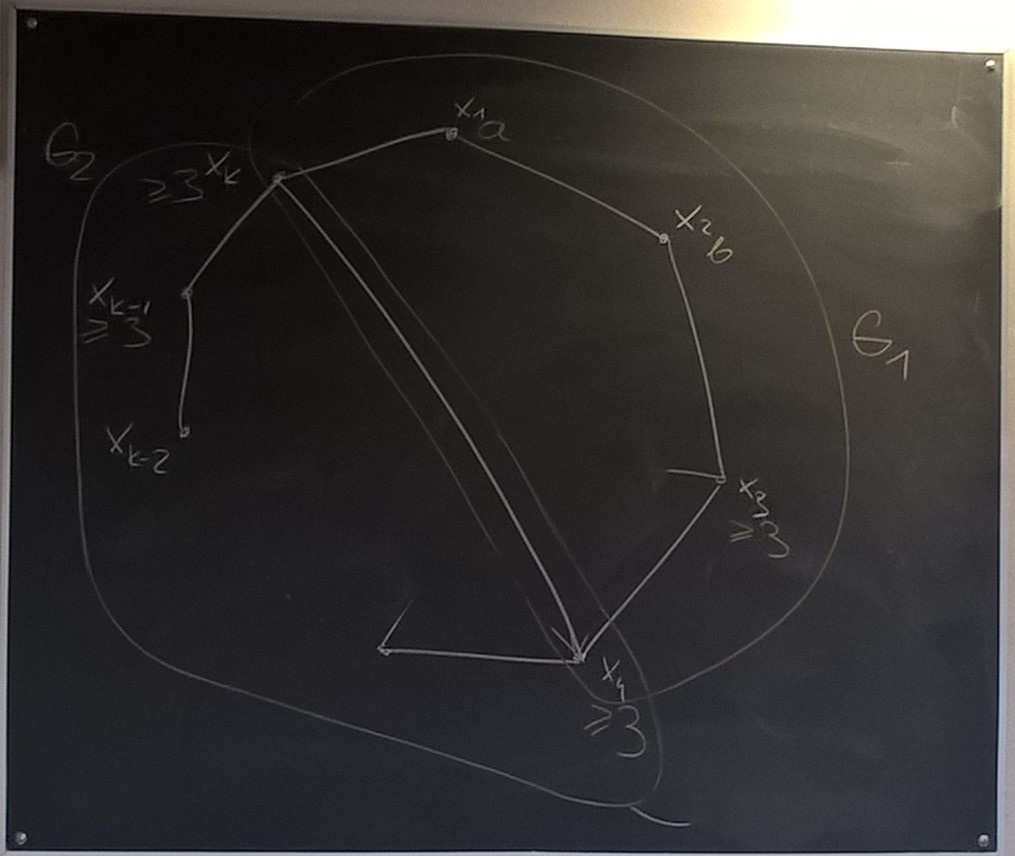
\includegraphics[scale=0.25]{Case1}
\end{center}
\begin{itemize}
\item[•]$G_1=$ graph bounded by $x_1x_2\ldots x_jx_k \rightarrow$ $L$-color $G_1$ by induction.
\item[•] $G_2=$ graph bounded by $x_kx_j\ldots x_{k-1} \rightarrow $ $L$-color $G_2$ by induction.
\item[•] $\rightarrow$ L-coloring of $G$. Note that after coloring $G_1$ some colors are not available for certain vertices of $G_2$, but there is enough left just to use the induction hypothesis for $G_2$.
\end{itemize}

\underline{Case 2}:

There are no edge $x_k x_j$, $j=2,\ldots,k-2$.
\begin{itemize}
\item Around $x_k$ we must have a sequence of triangles, since the interior is triangulated.
\item Let $N(X_k)=\{x_1,x_{k-1},y_1,\ldots,y_{\ell}\}$
\item Pick $c,d \in L(X_k)$, $c\neq d$, $c,d \neq a$.
\item Set $G'=G-x_k$ and note that $G' $ is a near-triangulation. 
\end{itemize}
\begin{center}
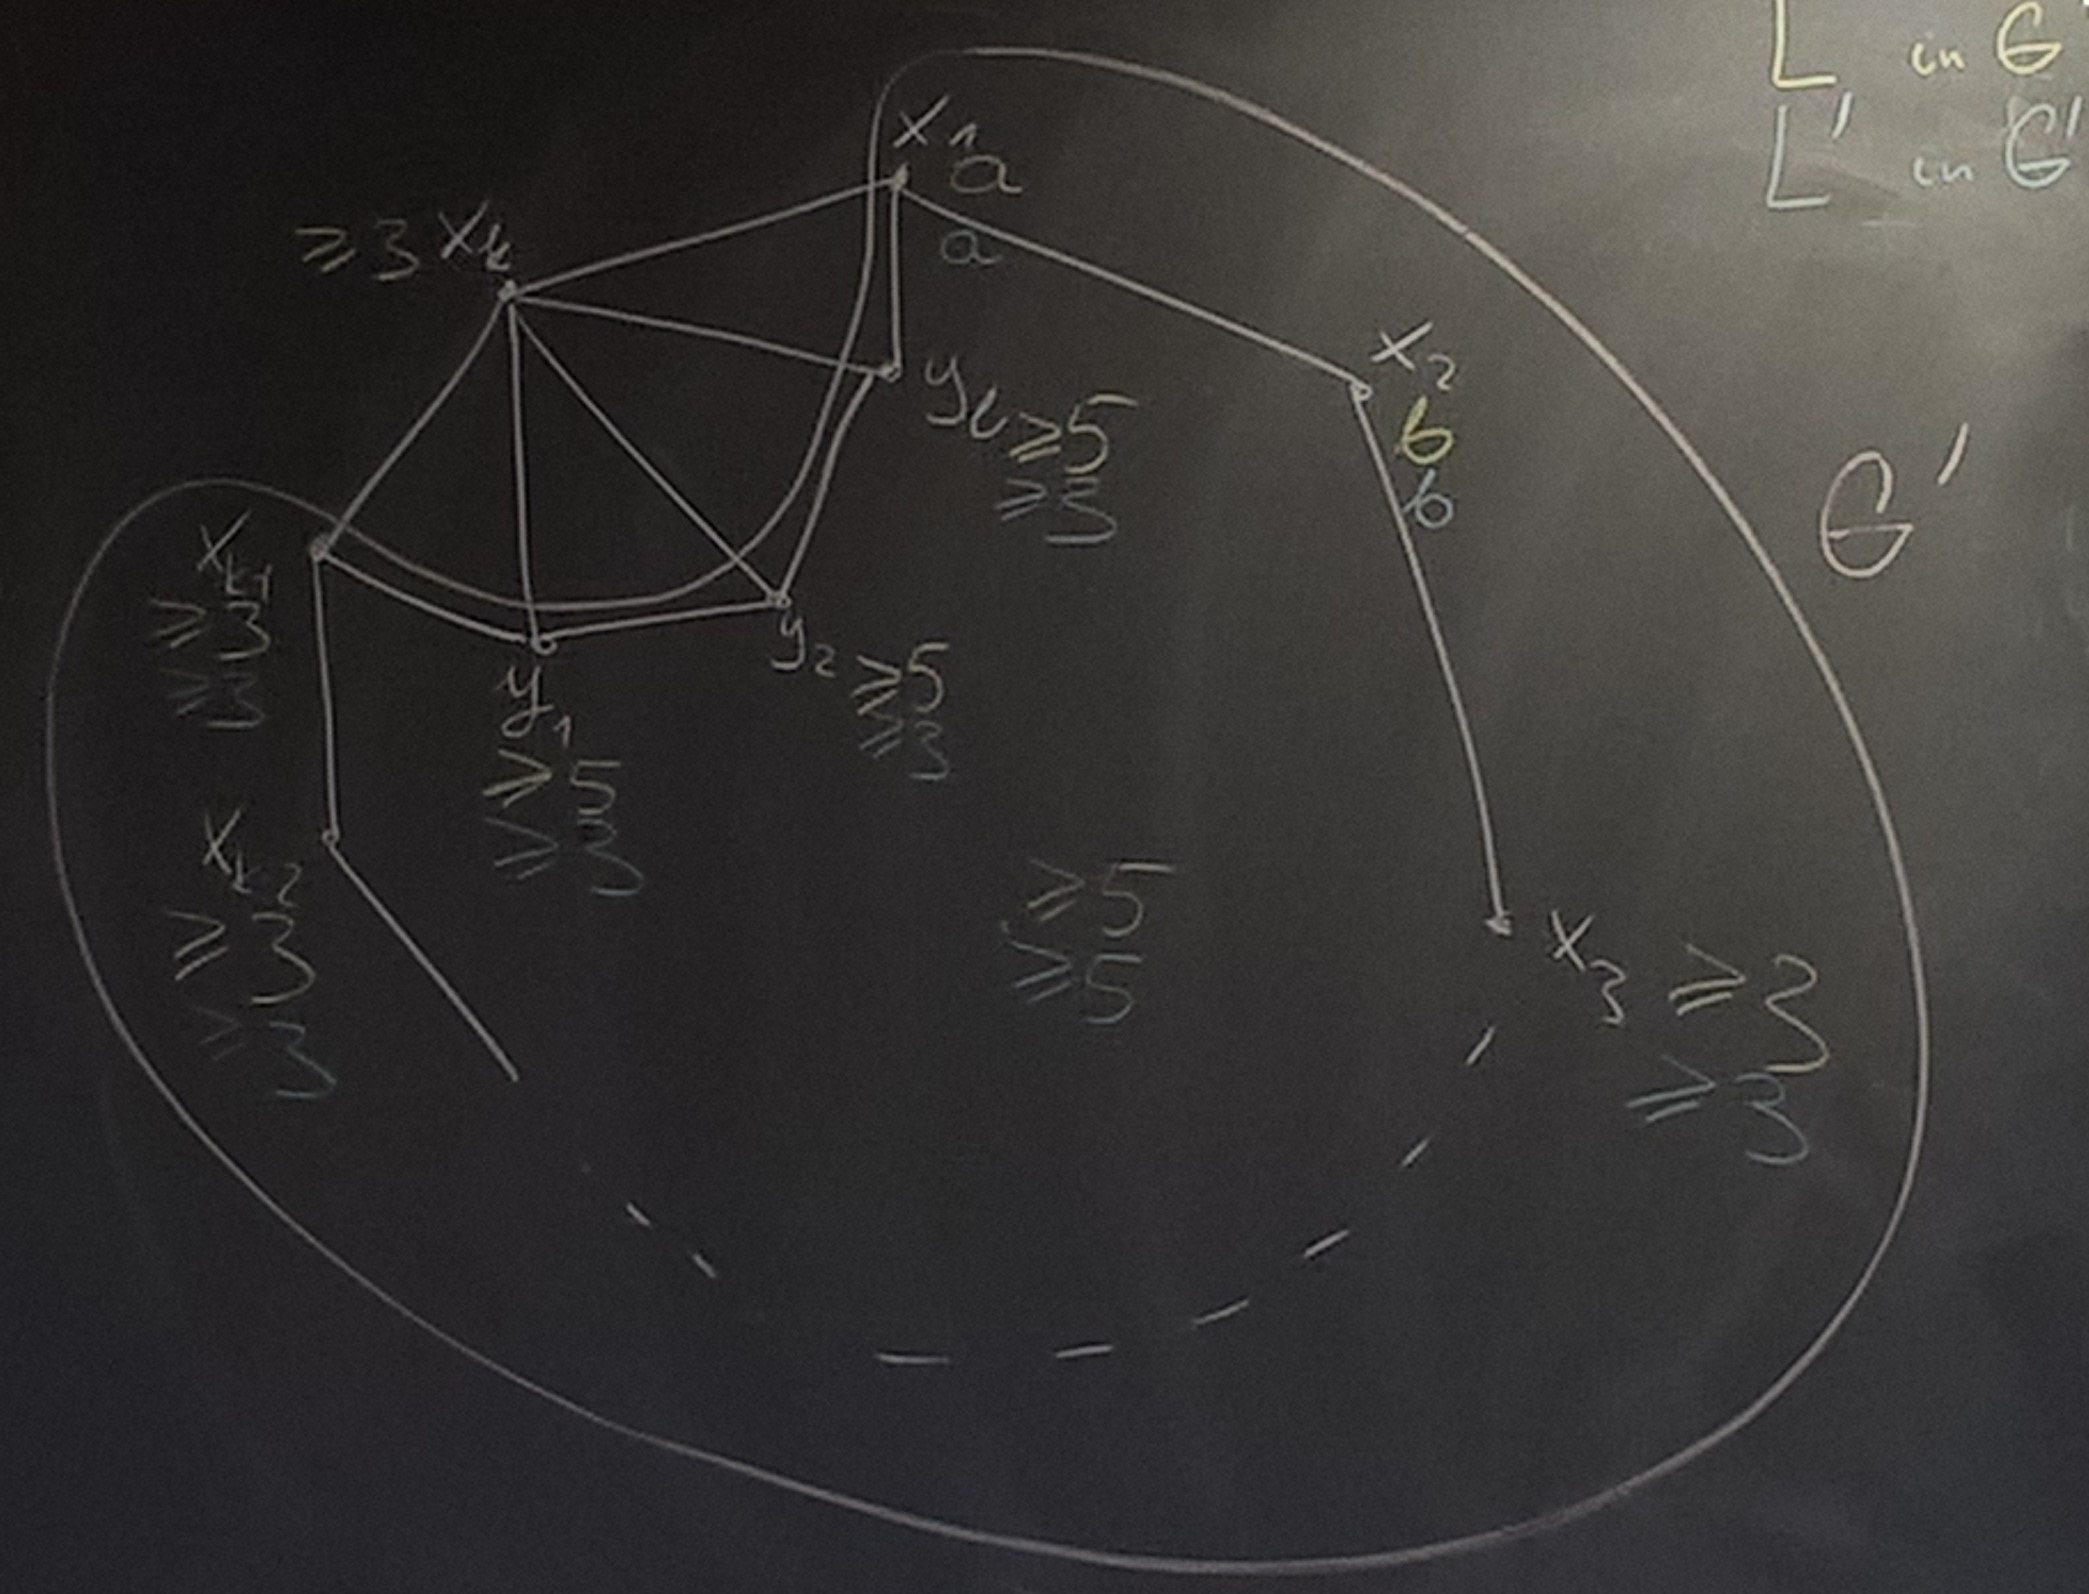
\includegraphics[scale=0.125]{Case2}
\end{center}
Consider the list:
\begin{align*}
L'(y_i)=L(y_i)\backslash \{c,d\} \ , \ L'(x)=L(x) \ \text{for any other} \ x \in G'
\end{align*}
$\leadsto$ There is a L'-coloring of $G'$ by induction.
\begin{align*}
c(y_i)\notin \{c,d\} \ , \ c(x_1) \notin \{c,d\}
\end{align*}
$\leadsto$ color $x_k$ with either $c$ or $d$ depending on $c(x_{k-1})$.
\end{proof}

\begin{remark}
There are planar not-4-list-colorable graphs. (Voigt '93 example with $\approx$ 300 vertices).
\end{remark}
\begin{remark}
Did not use Euler, upper/lower bounds. Only geometric properties.
\end{remark}
\subsubsection*{Application:
\underline{The art gallery problem}}

Suppose $P$ is a polygon in $\mathbb{R}^2$ with $n$ vertices.

\begin{example}
:
\begin{center}
\begin{tikzpicture}[
every node/.style={circle,inner sep=1pt,fill,draw}
]
\node (a) at (-4,0) {};
\node (b) at (-3.5,1) {};
\node (c) at (-3.5,-1) {};
\node (d) at (-2.5,1) {};
\node (e) at (-2.5,-1) {};
\node (f) at (-2,0) {};

\draw[thick] (a) -- (b);
\draw[thick] (a) -- (c) ;
\draw[thick] (b) -- (d);
\draw[thick] (d) -- (f);
\draw[thick] (e) -- (f);
\draw[thick] (e) -- (c);

\node (g) at (-1,-1) {};
\node (h) at (-0.5,1) {};
\node (i) at (0,0) {};
\node (j) at (0.5,1) {};
\node (k) at (1,-1) {};

\draw[thick] (h) -- (g);
\draw[thick] (g) -- (i);
\draw[thick] (h) -- (j);
\draw[thick] (j) -- (k);
\draw[thick] (k) -- (i);

\node (l) at (2,-1) {};
\node (m) at (2,1) {};
\node (o) at (3,1) {};
\node (p) at (3,0) {};
\node (q) at (4,0) {};
\node (r) at (4,1) {};
\node (s) at (5,1) {};
\node (t) at (5,-1) {};

\draw[thick] (l) -- (m);
\draw[thick] (m) -- (o);
\draw[thick] (o) -- (p);
\draw[thick] (p) -- (q);
\draw[thick] (q) -- (r);
\draw[thick] (r) -- (s);
\draw[thick] (s) -- (t);
\draw[thick] (t) -- (l);


\end{tikzpicture}
\end{center}

\end{example}

We assume the bounded region is the floor plan af an art gallery.
\begin{quote}
How many guards are needed to guard each point in sight?
\end{quote}

\begin{problem}
\begin{itemize}
\item Find a gallery with 6 vertices requiring $\geq 2$ guards.
\item Find a gallery with as few vertices as possible requiring $\geq k$ guards.
\end{itemize}
\end{problem}

\begin{observation}
There are $n$-vertex galleries requiring at least $\left \lfloor \frac{n}{3} \right \rfloor$ guards.
\end{observation}
\begin{center}
\begin{tikzpicture}[
every node/.style={circle,inner sep=1pt,fill,draw}
]
\node (a) at (-3.5,1.5) {};
\node (b) at (-3.25,0) {};
\node (c) at (-3,1) {};
\node (d) at (-2.5,1) {};
\node (e) at (-2.25,0) {};
\node (f) at (-2,1) {};
\node (g) at (-1,1) {};
\node (h) at (-0.75,0) {};
\node (i) at (-0.25,1.5) {};
\node (f') at (-2,1.5) {};
\node (g') at (-1,1.5) {};

\draw[thick] (a) -- (b);
\draw[thick] (b) -- (c) ;
\draw[thick] (c) -- (d);
\draw[thick] (d) -- (e);
\draw[thick] (e) -- (f);
\draw[dotted, thick] (f) -- (g);
\draw[thick] (g) -- (h);
\draw[thick] (h) -- (i);
\draw[dotted, thick] (f') -- (g');
\draw[thick] (i) -- (g');
\draw[thick] (a) -- (f');

\end{tikzpicture}
\end{center}

\begin{theorem}
Rephrasing the art gallery problem:

Every n-vertex gallery can be guarded by $\left \lfloor \frac{n}{3} \right \rfloor$ guards. ($\approx$ 70's Chvatal).
\end{theorem}

\begin{definition}
A planar embedding is called a \emph{polygon triangulation} if it is a near-triangulation and all vertices lie on the outer cycle.
\end{definition}

\begin{example}
"Polygon triangulated by diagonals"
\begin{center}
\begin{tikzpicture}[
every node/.style={circle,inner sep=1pt,fill,draw}
]
\node (a) at (-1,0) {};
\node (b) at (0,1) {};
\node (c) at (0,-1) {};
\node (d) at (1,0.75) {};
\node (e) at (1.25,-0.75) {};

\draw[thick] (a) -- (b);
\draw[thick] (a) -- (c);
\draw[thick] (c) -- (b);
\draw[thick] (d) -- (c);
\draw[thick] (b) -- (d);
\draw[thick] (c) -- (e);
\draw[thick] (d) -- (e);

\end{tikzpicture}
\end{center}
\end{example}

\begin{observation}
A triangulated polygon with n vertices has $2n-3$ edges, $n$ on the outer cycle and $n-3$ diagonals.
\end{observation}

\begin{observation}
Every triangulated polygon have a vertex of degree 2.
\end{observation}
\begin{proof}
The shortest diagonal cuts off such a vertex.
\end{proof}

\begin{observation}
Every triangulated polygon is 3-colorable.
\end{observation}
\begin{proof}
Take $v$ to be a vertex of degree 2. $G-v$ is a triangulated polygon. Color $G-v$ with 3 colors, the neighbours of $v$ will use 2 colors. Color $v$ with the spare color.
\end{proof}

\begin{proof}
Proof of Theorem 18:

\begin{itemize}
\item Let $G$ be planar polygon with $n$ vertices.
\item First triangulate using diagonals (Exercise: show that this is always possible).
\item The resulting triangular polygon is 3-colorable. 
\item Some color class will have $\leq \left \lfloor \frac{n}{3} \right \rfloor$ elements
\item Place guards at the vertices of that color.
\end{itemize}
\end{proof}
%%%%%%%%%%%%%%%%%%%%%%%%%%%%%%%%%%%%%%%%

\chapter{Chromatic polynomial}

\section{Definitions and simple properties}

In the last chapter we discussed the $4$-coloring problem for planar graphs. In the 1930s Birkhoff and Whitney had the idea that, instead of constructing one $4$-colouring for a planar graph, one could instead find a formula for the \emph{number} of $4$-colourings, and then use algebraic, analytical or whatever other tools to somehow prove that the formula always returns a strictly positive answer. The plan didn't work; but it lead to the notion of the chromatic polynomial.

\begin{definition} For a graph $G$ we define the chromatic function $P_G(t)$, $P(G,t)$ or $P(t)$, as 
\begin{align*}
P_G(t)&=\#\text{ of vertex colourings of G with colours }\lbrace 1,\dots ,t\rbrace\\
&=\left|\left\lbrace c:V(G)\to \lbrace 1,\dots ,t\rbrace : c\text{ is a colouring}\right\rbrace\right|
\end{align*}
\end{definition}

Note that the definition does not require that all the colors actually appear in the coloring, i.e. $c$ need not be surjective.

\begin{example}
\begin{enumerate}
\item[$\circ$] If $G=\overline{K_n}$, $P_G(t)=t^n$.
\item[$\circ$] If $G=K_n$, $P_G(t)=t(t-1) \cdots (t-(n-1))=t^{\underline{n}}$. (FIGURE)
\item[$\circ$] If $G=P_n$, $P_G(t)=t(t-1)^{n-1}$.
\item[$\circ$] If $G=\emptyset$, $P_G(t)=1$.
\item[$\circ$] Consider cycles, for instance $G=C_5$. (FIGURE) The direct method ends up with a small complication: we didn't keep track of whether $1$ and $4$ are coloured differently. We will return to this example later.
\item[$\circ$] The chromatic number can now be redefined as $\chi(G)=\min \lbrace k\in\mathbb{N} : P_G(k)>0\rbrace$.
\item[$\circ$] The $4$-colour theorem is equivalent to the statement that $P_G(4)>0$ for a planar graph $G$.
\end{enumerate}
\end{example}

Let us now try to generalize some of those examples.

\begin{lemma}
If $G$ is a tree with $n$ vertices, then
\begin{align*}
P_G(t)=t(t-1)^{n-1}.
\end{align*}
\end{lemma}
\begin{proof}
If $G$ is a single vertex, then $P_G(t)=t$. Pick a leaf $x\in V(G)$. After $G\setminus x$ has been coloured we can pick the color for $x$ in $t-1$ ways, so
\begin{align*}
P_G(t)=P_{G-x}(t)(t-1) = t(t-1)^{n-2}(t-1)=t(t-1)^{n-1}
\end{align*}
by induction.
\end{proof}

\begin{lemma}
The chromatic polynomial of a disjoint union is $P(G\sqcup H,t)=P(G,t)P(H,t)$.
\end{lemma}
\begin{proof}
Any pair (colouring of $G$, colouring of $H$) gives a colouring of $G\sqcup H$.
\end{proof}

Next we show that the chromatic function is indeed a polynomial.
\begin{proposition}
\label{prop:chromatic-partition}
Let $\pi_i(G)$ be the number of ways to partition $V(G)$ into exactly $i$ non-empty independent sets. For any graph $G$ with $n>0$ vertices
\begin{align*}
P_G(t)=\sum_{i=0}^n \pi_i(G) t^{\underline{i}}.
\end{align*}
\end{proposition}
\begin{proof}
The choice of a colouring with colours from $\lbrace 1,\dots , t\rbrace$ is the same as 
\begin{enumerate}
\item[$\circ$] choosing the number $i$ of colours that will actually be used,
\item[$\circ$] partitioning $G$ into $i$ independent sets; there are $\pi_i(G)$ ways to do this,
\item[$\circ$] colouring each part with a different colour; there are $t(t-1) \cdots  (t-(i-1))=t^{\underline{i}}$ ways.
\end{enumerate}
\end{proof}
\begin{example}
Let $G=P_3$. (FIGURE)
\begin{align*}
\pi_1 &=0\\
\pi_2 &= 1\quad ,\qquad 1-2-1\\
\pi_3 &= 1\quad ,\qquad 1-2-3\\
\pi_{\ge 4} &= 0
\end{align*}
Then
\begin{align*}
P_{P_3}(t)=\pi_2t^{\underline{2}}+\pi_3 t^{\underline{3}}=t(t-1)+t(t-1)(t-2)=t(t-1)^2
\end{align*}
\end{example}

From now on we call $P_G(t)$ the \emph{chromatic polynomial}. There are other ways to express $P_G(t)$ which also certify that the function is polynomial.

\begin{proposition}
\label{prop:chromatic-inclusion}
Suppose $G=(V,E)$ is a nonempty graph. Then
\begin{align*}
P_G(t)=\sum_{F\subseteq E} (-1)^{|F|} t^{c(F)}
\end{align*}
where $c(F)$ is the number of connected components of $(V,F)$.
\end{proposition}

Before the proof we quickly recall the Inclusion-Exclusion principle.

\begin{fact}
Suppose $A$ is a set, and $A_1,\dots, A_k$ are subsets of $A$. For any $X\subseteq \lbrace 1,\dots , k\rbrace$ define
\begin{align*}
A_X=\bigcap_{i\in X} A_i
\end{align*}
Then
\begin{align*}
\left| \overline{\bigcup_{i=1}^k A_i}\right| = \sum_{X\subseteq \lbrace 1,\dots , k\rbrace} (-1)^{|X|}|A_X|
\end{align*}
\end{fact}

\begin{example} Assume we have some ambient set $\mathcal{A}$, with  $A,B,C \subset \mathcal{A}$. (FIGURE)
Then we have
\begin{align*}
|A\cup B \cup C| &= |A|+|B|+|C| -|A\cap B|-|B\cap C|-|C\cap A| + |A\cap B\cap C|\\\\
|\overline{A\cup B\cup C}|&= |\mathcal{A} | - |A|-|B|-|C| +|A\cap B|+|B\cap C|+|A\cap C| -|A\cap B\cap C|
\end{align*}
\end{example}

\begin{proof}[Proof of Proposition~\ref{prop:chromatic-inclusion}]
Define $A=\lbrace g:V\to \lbrace 1,\dots ,t\rbrace\rbrace$ (this is the set of all functions, not just colourings). For every $e=xy\in E$, let $A_e=\lbrace g\in A : g(x)=g(y)\rbrace$. Now for $F\subseteq E$, let $A_F= \bigcap_{e\in F} A_e$. Clearly $|A_F|=t^{c(F)}$, because $g\in A_F$ must be constant on every component of $(V,F)$. But then we're done, as 
\begin{align*}
P_G(t)= \left| \overline{\bigcup_{e\in E} A_e}\right| \overset{Incl.-excl.}{=} \sum_{F\subseteq E} (-1)^{|F|} |A_F|
\end{align*}
\end{proof}

This will help us understand some coefficients of the chromatic polynomial.

\begin{notation}
If $P(t)$ is a polynomial, we write $[t^k]P(t)$ for the coefficient of $t^k$ in $P(t)$.
\end{notation}
\begin{lemma}
If $G$ is a graph with $n$ vertices and $m$ edges, then $P_G(t)$ is a polynomial of degree $n$, with
\begin{align*}
[t^n]P_G(t)=1\quad , \qquad [t^{n-1}]P_G(t)=-m
\end{align*}
\end{lemma}
\begin{proof}
By Proposition~\ref{prop:chromatic-inclusion} we have $c(F)\le n \Rightarrow \deg P_G \le n$. Now then $c(F)=n $ if and only if $F=\emptyset$, which implies $t^n$ appears exactly once in $P_G(t)$ with coefficient $(-1)^{|\emptyset|}=1$. Also, $c(F)=n-1$ if and only if $F=\lbrace e\rbrace$ is a single edge, which implies $t^{n-1}$ appears with coefficient $(-1)^{-1}m=-m$.
\end{proof}

\section{Deletion--contraction}

\begin{notation}
For $e\in E(G)$ we write: $G-e$ for $G$ with $e$ removed, and $G/e$ for $G$ with $e$ contracted. \\
(FIGURE)
\end{notation}
\begin{proposition}
(Deletion--contraction rule). If $e\in E(G)$, then
\begin{align*}
P_G(t)=P_{G-e}(t)-P_{G/e}(t)
\end{align*}
\end{proposition}
\begin{proof}
Let $e=xy\in E(G)$.
\begin{align*}
P_{G-e}(t)&=\#\text{ colourings with } c(x)\neq c(y) + \# \text{ colourings with } c(x)=c(y) \\
&= P_G(t)+P_{G/e}(t)
\end{align*}
\end{proof}
\begin{remark}
$|E(G-e)|=|E(G)|-1$ and $|V(G/e)|=|V(G)|-1$, so we could define $P_G(t)$ recursively
\begin{align*}
P_G(t) = \left\lbrace \begin{array}{ll}
t^{|V(G)|} & \text{if } G \text{ has no edges}\\
 & \\
P_{G-e}(t)-P_{G/e}(t) & \text{if } e\in E(G)
\end{array} \right.
\end{align*}
\end{remark}

\begin{example} $G$ is a graph on $5$ vertices, and we run the above.
(FIGURE)
\begin{align*}
= t(t-1)^3-2t(t-1)^2(t-2)(t-2)+t(t-1)(t-2)
\end{align*}
\end{example}
\begin{example}
$P(C_n,t)=P(P_n,t)-P(C_{n-1},t)$. We have
\begin{align*}
P(P_n,t)&= t(t-1)^{n-1}\\
P(C_3,t)&=t(t-1)(t-2)
\end{align*}
Now one can prove by induction that $P(C_n)=(t-1)^n+(-1)^n(t-1)$. In particular
\begin{align*}
P(C_n,2)=1+(-1)^n= \left\lbrace \begin{array}{ll}
2, & 2\mid n\\
0, & 2\nmid n
\end{array}\right.
\end{align*}
which agrees with what we know about $\chi(C_n)$.
\end{example}

The deletion-contraction rule has many interesting consequences. 

\begin{proposition}
Let $G$ be a graph with $n>0$ vertices, $m$ edges and $c$ connected components. The coefficients of $P_G(t)$ alternate in signs, i.e.
\begin{align*}
P_G(t)=\sum_{i=0}^n (-1)^i c_i(G)t^{n-i}
\end{align*}
where $c_i(G)\ge 0$. Moreover $c_i(G)=0$ for $i>n-c$ and $c_{n-c}(G)\neq 0$.
\end{proposition}
Simply put, this proposition states that the chromatic polynomial has the form
\begin{align*}
P_G(t)=t^n-mt^{n-1}+c_2(G)t^{n-2}-\cdots + (-1)^{n-c}c_{n-c}(G)t^c.
\end{align*}
It is very easy to come up with a proof by induction, and we leave it as an exercise. It will be instructive for the future to phrase the proof slightly differently.
\begin{proof} Deleting an edge keeps the sign, and contracting an edge changes the sign. Successive contraction--deletion splittings produce a tree which looks like this:

(FIGURE)

We chose to continue with the splittings until we reach a graph with no edges, that is one of the $\overline{K_i}$, $1\le i \le n$. Every branch ending with $\overline{K_i}$ contributes
\begin{align*}
(-1)^{n-i}t^i
\end{align*}
to the chromatic polynomial. That is because the path from $G$ to $\overline{K_i}$ contains $n-i$ contractions, i.e. $n-i$ sign changes. It means that the proposition holds with
\begin{align*}
c_i(G)=\# \text{ of branches ending with } \overline{K_i}
\end{align*}
and clearly $c_i(G)\geq 0$.

To prove that $c_i(G)=0$ for $i>n-c$ note that no branch of the tree ends with a graph on less than $c$ vertices. Moreover, there is at least one branch with ends exactly with $K_c$ (apply contractions all the time), so $c_{n-c}(G)>0$.
\end{proof}


\section{Coefficient sequence}

As a small side remark, the behaviour of the coefficient sequences of chromatic polynomials is the subject of active research and is the topic of many conjectures and theorems. Most of that work takes place in the general context of \emph{matroids} and their \emph{characteristic polynomials}, of which the chromatic polynomial is a special case. Here is a very fresh result which proves a conjecture of Read from 1968. The proof uses techniques from algebraic geometry and singularity theory.

\begin{theorem} \emph{(June Huh, 2010)}
Suppose $G$ is connected with chromatic polynomial
$$P_G(t)=t^n-c_1t^{n-1}+c_2t^{n-2}-\cdots +(-1)^{n-1}c_{n-1}t.$$
Then the sequence $(1,c_1,c_2,\dots,c_{n-1})$ is log-concave, which means
$$c_{i-1}c_{i+1}\leqslant c_i^2 \quad \text{for all } i.$$
In particular, it is unimodal, which means
$$1 \leqslant c_1 \leqslant c_2 \leqslant \cdots \leqslant c_{k-1} \leqslant c_k \geqslant c_{k+1} \geqslant \cdots \geqslant c_{n-1}, \quad \text{for some } k.$$
\end{theorem}


\begin{remark} We can prove $1 \leqslant c_1 \leqslant c_2 \leqslant \cdots \leqslant c_{\lfloor \frac{1}{2}(n-1)\rfloor}$.
\\ If $G$ is a tree, then
$$P_G(t)=t(t-1)^{n-1}=\sum_{i=0}^{n-1} {n-1 \choose i}(-1)^it^{n-i}\cdot t=t^n-{n-1 \choose 1}t^{n-1}+{n-1 \choose 2}t^{n-2}-\cdots.$$
The sequence $(1,c_1,c_2,\dots)$ is $(1,{n-1 \choose 1},{n-1 \choose 2},\cdots)$, and it is increasing up to the middle term.
\\ Now suppose that $G$ is connected, but not a tree. Then, by definition of a tree, there is an edge $e\in E(G)$ such that $G-e$ is still connected. For $i\leqslant \frac{1}{2}(n-1)$ we notice that
$$P_G(t)=P_{G-e}(t)-P_{G/e}(t) \Longrightarrow c_{i-1}(G)=c_{i-1}(G-e)-(-c_{i-2}(G/e))=c_{i-1}(G-e)+c_{i-2}(G/e).$$
We know $i\leqslant \frac{1}{2}(n-1)$ and $i-1 \leqslant \frac{1}{2}(n-2)=\frac{1}{2}(|V(G/e)|-1)$, hence by induction 
 $$c_{i-1}(G)\leqslant c_i(G-e)+c_{i-1}(G/e)=c_i(G)$$
which ends the induction step.
\end{remark}


\section{Counting acyclic orientations}

What else does the chromatic polynomial count? And how?

\begin{definition} An \emph{orientation} of $G$ is a choice  of direction for every edge. This gives a directed graph. If $G$ has $m$ edges, then it has $2^m$ possible orientations (which might also be isomorphic).
\end{definition}

\begin{definition} An orientation is \emph{acyclic} if it has no closed directed walk. Let $a(G)$ be the number of acyclic orientations of $G$.
\end{definition}

\begin{theorem} \emph{(Stanley, 1973)}
If $G$ has $n$ vertices, then $a(G)=(-1)^nP_G(-1)$.
\end{theorem}

\begin{example}
\begin{itemize}
\item $G$ is a tree with $n$ vertices, then
$$a(G)=2^{n-1}=(-1)^n(-1)(-1-1)^{n-1}=(-1)^nP_G(-1),$$
\item $G$ is a cycle on $n$ vertices, then
\begin{align*}
a(G)&=2^n-2, \\
(-1)^nP_G(-1)&=(-1)^n[(-2)^n+(-1)^n(-2)]=(-1)^n[(-1)^n(2^n-2)]=a(G),
\end{align*}
\item $G=K_n$, then
\begin{align*}
(-1)^nP_G(-1)&=(-1)^n(-1)^{\underline{n}}=(-1)^n(-1)(-1-1)(-1-2)\cdots (-1-(n-1))=(-1)^n(-1)^nn!.
\end{align*}
An acyclic orientation is the same as ordering the vertices $v_1,v_2,\dots,v_n$ (there are $n!$ possibilities to do this) and then choosing the orientation
$$v_i\longrightarrow v_j, \quad \text{whenever } i>j.$$
\end{itemize}
\end{example}

\begin{proof}
Take $e=xy \in E(G)$. Write $a^+(G-e),a^-(G-e),a^0(G-e)$ for the number of acyclic orientations of $G-e$ such that:
\begin{itemize}
\item There is a directed walk in $G-e$ from $x$ to $y$ ($a^+$),
\item There is a directed walk in $G-e$ from $y$ to $x$ ($a^-$),
\item There is no directed walk either way ($a^0$).
\end{itemize}

We prove a few claims about these quantities:
\begin{itemize} 
\item $a(G-e)=a^+(G-e)+a^-(G-e)+a^0(G-e)$. 
An acyclic orientation in $G-e$ cannot have directed walks $x\longrightarrow y$ and $y\longrightarrow x$ at the same time. These three sets are therefore disjoint and they give all the possibilities.

\item $a(G/e)=a^0(G-e)$. 
Take an orientation of $G-e$ with no walk $x\longrightarrow y$ or $y\longrightarrow x$. For any $z\in N_{G-e}(x)\cap N_{G-e}(y)$, the edges $xz$ and $yz$ have the same orientation (if not, there would be a walk $x\longrightarrow z\longrightarrow y$ or $y\longrightarrow z\longrightarrow x$), hence either  
$$x\longrightarrow z \text{ and } y\longrightarrow z$$
or
$$z\longrightarrow x \text{ and } z\longrightarrow y.$$
The orientation of $G-e$ determines then an orientation of $G/e$ (the edges $xz$ and $yz$ are compatible under the contraction). This orientation is also acyclic (a directed walk from $xy$ to itself would imply a directed walk in $G-e$ from $x$ or $y$ to $y$ or $x$). This also works vice versa.
\\ The idea here was that 
$$\text{Closed walks in } G/e = \text{Walks } x\longrightarrow y \text{ or } y\longrightarrow x \text { in } G-e.$$

\item $a(G)=a^+(G-e)+a^-(G-e)+2a^0(G-e)$. 
For the first two terms there is only one way to extend the orientation of $G-e$ without closing a cycle in $G$. In the last case the edge $xy$ can be oriented both ways, since we don't have a walk from $x$ to $y$ or from $y$ to $x$.
\end{itemize}

By these three claims we obtain
\begin{align*}
a(G)&=a^+(G-e)+a^-(G-e)+2a^0(G-e)= \\
&= a^+(G-e)+a^-(G-e)+a^0(G-e)+a^0(G-e)= \\
&= a(G-e)+a^0(G-e)= \\
&= a(G-e)+a(G/e)
\end{align*}
We complete the proof by using induction:
\begin{itemize}
\item $G=K_1$, then $a(G)=1=(-1)^1P_{K_1}(-1)$,
\item Pick an edge $e\in E(G)$, then (by induction assumption)
\begin{align*}
a(G)&=a(G-e)+a(G/e)= \\
&= (-1)^nP_{G-e}(-1)+(-1)^{n-1}P_{G/e}(-1)= \\
&= (-1)^n[P_{G-e}(-1)-P_{G/e}(-1)]= \\
&= (-1)^nP_G(-1)
\end{align*}
\end{itemize}
\end{proof}

Stanley's theorem is, again, just the tip of an iceberg known as \emph{duality} in matroid theory. It has many generalizations.


\section{Chromatic roots}

Let's try to wrap up this chapter by going back to the original question of Birkhoff and Whitney: is there something interesting to say about the set of points where the chromatic polynomial is positive? Or, alternatively, is there something interesting to say about their roots?

\begin{definition} $\alpha \in \mathbb{C}$ is a \emph{chromatic root} if $P_G(\alpha)=0$ for some graph $G$.
\end{definition}

Here are some very simple observations about chromatic roots.

\begin{observation}
\begin{enumerate}
\item Every natural number is a chromatic root,
\item For any $G$ different from the empty graph, $P_G(0)=0$,
\item For any $G$ with at least one edge, $P_G(1)=0$,
\item If $\alpha$ is a chromatic root, then so is $\alpha+1$ (because $P_{G+K_1}(\alpha+1)=(\alpha+1)P_G(\alpha)$),
\item The set of chromatic roots is countable (as a subset of the algebraic numbers).
\end{enumerate}
\end{observation}

The next proposition is less obvious (at least one of its parts). The proof is an appropriate adaptation of the deletion-contraction principle (again).

\begin{proposition} There is no chromatic root in $(- \infty, 0)\cup (0,1)$.
\end{proposition}

\begin{proof}
$\alpha <0$ is not a root of $P_G(t)$, since the coefficients of the polynomial have alternating signs.

Take $\alpha \in (0,1)$. Because $P_{G\sqcup H}(t)=P_G(t)P_H(t)$, it suffices to prove that $P_G(\alpha)\neq 0$ for any connected graph. Apply the deletion-contraction rule to $G$, in such a way that all the intermediate graphs are connected. At each step, either $G$ is a tree (and we stop splitting) or there is an edge $e\in E(G)$ such that $G-e$ is still connected.

A branch of this splitting process with $i$ contractions
\begin{itemize}
\item ends with an $(n-i)$-vertex tree,
\item introduces a sign of $(-1)^i$,
\item contributes $t(t-1)^{n-i-1}$ to $P_G(t)$.
\end{itemize}
Define $d_i$ as the number of branches ending with an $(n-i)$-vertex tree, then
$$P_G(t)=\sum d_i(-1)^it(t-1)^{n-i-1},$$
and of course we have $d_i\geqslant 0$.
Evaluate $P_G(\alpha)$ for $\alpha \in (0,1)$:
$$sgn\{d_i(-1)^i\alpha (\alpha-1)^{n-i-1} \}=(-1)^i\cdot 1\cdot (-1)^{n-i-1}=(-1)^{n-1},$$
which means that all monomials in $P_G(\alpha)$  evaluate to positive or all evaluate to negative, hence $P_G(\alpha) \neq 0$ as $d_i>0$ for at least one $i$. 
\end{proof}

This time we applied the deletion-contraction principle until we reached trees, and not edge-less graphs.

It actually gets much better.

\begin{theorem} \emph{(Jackson, Thomassen)}
There are no chromatic roots in $(- \infty, 0)\cup (0,1)\cup (1,\frac{32}{27}).$ Moreover, the constant $\frac{32}{27}$ is optimal. 
\end{theorem}

It is also known (Sokal) that chromatic roots are a dense subset of the complex numbers. In the context of planar graphs the best we have now is:

\begin{theorem} \emph{(Birkhoff, Lewis)}
If $G$ is planar, then $P_G(t)>0$ for all $t\in [5,\infty)$.
\end{theorem}

It is conjectured that if $G$ is planar, then $P_G(t)>0$ for all $t\in [4,\infty)$. Even with the $4$-color theorem ($P_G(4)>0$) we still don't know if there is a \emph{planar} chromatic root in $(4,5)$. So, in a sense, Birkhoff's and Whitney's analytic--algebraic plan turned out to be much harder than the original combinatorial problem.

\section{Exercises}

\begin{enumerate}
\item What is $\min\{P_G(4)~:~G\ \mathrm{is\ planar}\}$\ ?
\item Find the chromatic polynomial of
\begin{itemize}
\item The $2\times n$ grid $K_2\square P_n$.
\item The wheel $W_n$.
\item $K_n-e$, the complete graph with one edge removed.
\item $P_n[K_m]$ (graph substitution, see TODO).
\item The disjoint union of two graphs.
\item $K_2 \square P_n$.
\end{itemize}
\item  Let $G,G_1,G_2$ be graphs such that $G=G_1 \cup G_2$ and $G_1 \cap G_2 \simeq K_k$ for some $k\geqslant 0$. Then
$$P_G(t)=\frac{1}{t^{\underline{k}}}P_{G_1}(t)P_{G_2}(t).$$
\item Let $P'_G(t)$ denote the number of colorings of $G$ with \emph{exactly} $t$ colors $1,\ldots,t$ appearing, i.e. such that the color assignment $c:V(G)\to\{1,\ldots,t\}$ is surjective. Show that $P'_G(t)$ is not a polynomial for any graph $G$.
\item If $G$ is a graph with chromatic polynomial $P(t)$, construct a graph with chromatic polynomial
\begin{itemize}
\item $tP(t-1)$,
\item $(t-1)P(t)$,
\item $P(t)^3$,
\item $P(t)^2/t$.
\end{itemize}
\item Let $G$ be a graph with $n$ vertices, $m$ edges and $r$ triangles. Show that $[t^{n-2}]P_G(t)={m\choose 2}-r$.
\item Let $G$ be a graph with $n$ vertices, $m$ edges and chromatic polynomial $P_G(t)=\sum_{i=0}^na_it^{n-i}$. Prove that $|a_i|\leq{m\choose i}$.
\item Where does the term \textit{log-concave} sequence come from? Prove that a log-concave sequence of positive real numbers is unimodal.
\end{enumerate}

\chapter{Interlude --- graph coloring game}

We fix a graph $G$ and a set of colors $C$.

Two players, Alice and Bob, take turns coloring one vertex of $G$ at a time, using a color from $C$, and so that any adjacent vertices which are already colored have different colors. Alice starts. 

Alice wins when all vertices of $G$ are colored (her aim is to color the whole graph). Bob wins if some player has no legal move (he is an adversary trying to stop Alice).

\subsection*{Some games to play}
\medskip

Who has a winning strategy?
\begin{itemize}
\item $G=P_3$, $C=\{1,2\}$
\item $G=P_6$, $C=\{1,2\}$
\item $G=C_6$, $C=\{1,2\}$
\item $G=C_8$, $C=\{1,2,3\}$
\item $G=Q_3$, $C=\{1,2,3,4\}$
\item $G=Q_3$, $C=\{1,2,3\}$
\item $G$ is the tree below, and $C=\{1,2,3\}$
%\begin{center}
%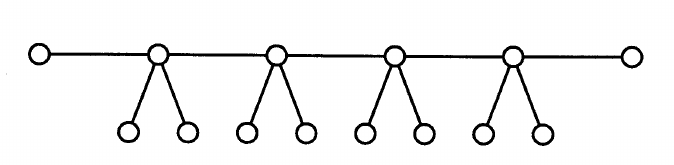
\includegraphics[scale=0.5]{mf4.png}
%\end{center}
\item Come up with your own pair $(G,C)$, where Bob has a winning strategy, and you think this strategy is not easy to find. Play the game instances you came up with against your classmates.
\end{itemize}

\subsection*{Questions}
\medskip
Let $\chi_g(G)$ be the smallest number of colors $k$ for which Alice has a winning strategy in the coloring game on the graph $G$ with $k$ available colors. We call it the \emph{game chromatic number} of $G$.

\begin{itemize}
\item Prove that $\chi(G)\leq \chi_g(G)\leq \Delta(G)+1$.
\item Find bipartite graphs with arbitrarily large $\chi_g$.
\item Describe all graphs with $\chi_g(G)\leq 2$.
\end{itemize}

\chapter{Edge coloring}

\section{Definitions and examples}

Until now we concentrated on coloring vertices of graphs. In this chapter we briefly address the concept of edge-coloring.

\begin{definition}
An \emph{edge-coloring} of $G=(V,E)$ is a function $f:E\rightarrow C$ (for some set of colors $C$) such that if two edges $e_1$, $e_2$ have a common endpoint then $f(e_1)\neq f(e_2)$. The \emph{edge chromatic number} (\emph{chromatic index}) $\chi'(G)$ is the smallest $k$ such that $G$ has an edge-coloring with colors $\{1,\dots,k\}$.
\end{definition}

[FIGURE]

\begin{example}[Cycles]
The $n$-cycle $C_n$ can be edge-colored with $2$ colors when $n$ is even and requires $3$ colors when $n$ is odd, therefore
$$\chi'(C_n)=
\begin {cases}
2 & 2|n\\
3 & 2\not|n
\end {cases}$$
\end{example}

\begin{example}[Scheduling]
Let $G$ be a bipartite graph whose two parts are $Classes$ and $Teachers$. There is an edge $tc$ if teacher $t$ is supposed to teach class $c$. How many time slots do we need to allocate to schedule all lessons?

[FIGURE]

The answer is $\chi'(G)$. Each color represents one time slot, and the edge-coloring condition guarantees that no teacher and no class is required to show up at two different events at the same time.
\end{example}

\begin{example}[Complete graphs]
As we all know a full soccer season in a league with $2k$ teams consists of $2k-1$ rounds. Each team plays exactly once in each round, and each pair meets once. This is just the statement that
$$\chi'(K_{2k})=2k-1.$$
Indeed, each color represents one week of the season, and the edges of a particular color determine the pairs of teams playing that week. We can of course make a more general statement about the edge-chromatic numbers of complete graphs:
$$\chi'(K_n)=
\begin {cases}
n-1 & 2|n\\
n & 2\not|n
\end {cases}$$
[FIGURE]

It is not hard to find a coloring. It $n=2k-1$ is odd, arrange the vertices into a regular $n$-gon. Choose a color class consisting of $k$ parallel edges (one vertex is left out). This color class has $n$ possible rotations. These rotations cover all edges of $K_n$. This is an edge-coloring with $n$ colors,so $\chi'(K_n) \leq n$. For an upper bound, take any edge-coloring of $K_n$. The color class $1$ must miss some vertex $v$. Since all edges incident to $v$ require $n-1$ colors, we get at least $1+(n-1)=n$ colors in total.

If $n=2k$ is even arrange $n-1$ vertices in a regular $(n-1)$-gon and place one vertex at the origin. Use $k-1$ parallel edges and one edge from the origin to the vertex on the perimeter being left out. This is one color class, and the $n-1$ rotations of this class form a desired edge-coloring. The upper bound is obvious.
\end{example}

\begin{lemma} 
$\chi'(G) \geq \Delta(G)$
\end{lemma}
\begin{proof}
We need at least $\Delta(G)$ colors just to color the edges incident to the vertex of maximum degree.
\end{proof}


\section{Basic properties}

As with vertex-colorings, also edge-colorings can be expressed using other familiar language of graph theory. In fact edge-colorings can be seen as a special case of vertex-colorings.

\begin{definition}
A \emph{matching} in $G$ is a set of edges, no two of which have a common endpoint.
\end{definition} 

This is a very important concept in graph theory. Equivalently, a matching in $G$ is a $1$-regular subgraph of $G$. 

\begin{proposition}
Let $G=(V,E)$ be a graph.
\begin{itemize}
\item If $f$ is an edge-coloring of $G$ then every color class $f^{-1}(c)$ is a matching.
\item An edge-coloring with $k$ colors is the same as a partition of $E$ into $k$ matchings.
\item For any two colors $c_1,c_2\in C$, $c_1\neq c_2$, the edge set $f^{-1}(c_1)\cup f^{-1}(c_2)$ is a disjoint union of cycles and paths.
\end{itemize}
\end{proposition}
\begin{proof}
The first two parts are clear. For the last one, note that in $f^{-1}(c_1)\cup f^{-1}(c_2)$ every vertex is of degree at most $2$.
\end{proof}

\begin{definition}
Let $G=(V,E)$. The \emph{line graph} $L(G)$ has vertex set $E$, and $e_1$, $e_2$ are adjacent in $L(G)$ if they share a common vertex in $G$.
\end{definition}

\begin{example}
The line graph simply keeps track of the incidence relation between the edges of $G$. 

[FIGURE]
\end{example}

All the entries in the following glossary should now be completely obvious. It translates edge-coloring notions into their vertex-coloring counterparts.

\begin{center}
\begin{tabular}{l|l}
Edges of $G$ & Vertices of $L(G)$ \\
\hline
{edge in $G$} & {vertex of $L(G)$} \\
{matching in $G$} & {independent set in $L(G)$} \\
{edge-coloring of $G$} & {vertex coloring of $L(G)$} \\
{$\chi'(G)$} &  {$\chi(L(G))$} 
\end{tabular}
\end{center}

We have $\omega(L(G))\geq \Delta(G)$ because all edges incident to a fixed vertex $v$ induce a clique in $L(G)$. That implies $\chi'(G)=\chi(L(G))\geq \omega(L(G))\geq \Delta(G)$ which we already knew. Moreover $\Delta(L(G))= \max_{uv\in E(G)}(deg_G(u)+deg_G(v)-2)\leq 2\Delta(G)-2$, so $\chi'(G)=\chi(L(G)) \leq \Delta(L(G))+1\leq 2\Delta(G)-1$. Altogether this shows
$$\Delta(G)\leq \chi'(G) \leq 2\Delta(G)-1.$$
In fact the situation is much ``better'', in that the uncertainty interval for $\chi'(G)$ is as short as possible without being trivial. There are only two possibilities for $\chi'(G)$\ !
\begin{theorem}
\label{thm:vizing}
(Vizing '64) For any graph $G$ we have
$$\Delta(G)\leq \chi'(G) \leq \Delta(G)+1.$$
\end{theorem}
\begin{remark}
In some older literature graphs with $\chi'(G)=\Delta(G)$ are called ``Class 1'' and those with $\chi'(G)=\Delta(G)+1$ are called ``Class 2''. (Un?)surprisingly it is still NP-hard to recognize if $\chi'(G)=\Delta(G)$ or $\chi'(G)=\Delta(G)+1$, even for graphs with $\Delta(G)=3$.
\end{remark}

In the next section we will prove that bipartite graphs are Class 1. The main tool is one of the most classical results in combinatorics --- Hall's marriage theorem, which we discuss next.


\section{Hall's marriage theorem and applications}

Here is a version of the question commonly known as \emph{Hall's marriage problem}, first studied by Hall in the 1930s. We have a number of boys and girls, and each girl fancies some of the boys. We want to pair them up so that each girl is in a couple with a boy she fancies. Under what conditions is such a pairing possible?\footnote{As dictated by the political correctness of the 21st century, we ignore the preferences of the boys and we let some of the boys to leave without a girl.}

There are obvious necessary conditions that must be met for this to work. For example, each girl must fancy at least one boy. Of course this is not enough, because two girls might desire only one and the same boy. We can avoid this situation with a more general necessary condition: every set of $k$ different girls must altogether like at least $k$ different boys, for each $k\geq 1$. Hall's marriage theorem states that this necessary condition is also sufficient. Here it is in the language of bipartite graphs.

\begin{theorem}
(Hall 1935) Suppose $G$ is a bipartite graph with parts $V(G)=A\cup B$, such that for every $X\subseteq A$ we have:
$$|\bigcup_{x\in X}N_G(x)|\geq |X|.$$
Then $G$ has a matching of size $|A|$.
\end{theorem}
\begin{proof}
Write $N_G(X)=\bigcup_{x\in X} N_G(x)$ and let $n=|A|$. The proof is by induction on $n$. If $n=0$ there is clearly nothing to do. Otherwise we split the proof into two cases.

\begin{itemize}
	\item Suppose that for any $\emptyset\neq X\subsetneq A$, $|N_G(X)|\geq|X|+1$, so the inequality always holds with a surplus. Take any $a\in A$, $b\in N_G(a)$, match them, and use the inductive assumption in the graph $G'=G[A-a,B-b]$. This is possible because for any $X'\subseteq A-a$ we have $|N_{G'}(X)|\geq |N_G(X)|-1 \geq (|X|+1)-1=|X|$.

	\item Now suppose there is a set $\emptyset\neq X\subsetneq A$ with $N_G(X)=|X|$. Then by induction we find appropriate matchings in $G'=G[X,N(X)]$ and $G''=G[A-X,B-N(X)]$ and join them to form a matching in $G$. The only nontrivial fact to be checked is that $G''$ satisfies the inductive assumption. Pick any $Y\subseteq A-X$. Then $$|Y|+|X|=|Y\cup X|\leq|N_G(Y\cup X)|=|N_G(X)|+|N_G(Y)\cap(B-N(X))|=|X|+|N_G(Y)\cap(B-N(X))|.$$ 	It follows that $|Y|\leq |N_G(Y)\cap(B-N(X))| = |N_{G''}(Y)|$ as required.
\end{itemize}
[FIGURES]
\end{proof}

The marriage theorem has many interesting applications, especially to regular configurations, often combined with a counting argument as below.

\begin{example}
Split the standard 52 card deck into 13 piles of 4 cards each. Regardless of the splitting we can choose 1 card from each pile, so that we have one card of each rank: $A,2,3,\dots,K$.

To see this, construct a bipartite graph $G$ where the two parts are $R$ (ranks) and $P$ (piles). There is an edge $rp\in E(G)$ if pile $p$ contains a card of rank $r$. A matching in $G$ with 13 edges determines a bijection $P\longleftrightarrow R$. All we need to do is find such a matching with Hall's theorem.

[FIGURE]

Take any subset $X\subseteq R$ of ranks. This subset represents $4\cdot|X|$ actual cards. Since each plie has size 4, these $4|X|$ cards must occupy at least $|X|$ piles. But that means that the ranks in $X$ are adjacent to at least $|X|$ piles in $|P|$ in total, which is exactly the statement $|N_G(X)|\geq|X|$.
\end{example}

Note that in the above example cards of one rank (say all aces) can be distributed to less than 4 piles, so it would be more convenient to represent the situation with a \emph{multigraph}, where multiple edges between vertices are allowed.

[FIGURE]

This is the only part of these notes where we use the concept of a multigraph. Without going into too much formalism let us just note that the multiple edges adjacent to a vertex all contribute to its degree, so in the example above each vertex in $R$ has degree 13 and each vertex in $P$ has degree $4$ (in the multigraph sense).

Repeating a very similar argument yields the next theorem.

\begin{theorem}
\label{thm:chip-d-regular}
If $G=(V,E)$ is a $d$-regular bipartite multigraph, then $\chi'(G)=d$.
\end{theorem}
\begin{proof}
Denote by $V=A\cup B$ the parts of the bipartition. Then $|A|=|B|=n$, because $d\cdot |A|=|E|=d\cdot |B|$. 

We prove the theorem by induction. If $d=1$ then $G$ itself is a matching, so we are done. Let $d\geq 2$. We will first use Hall's theorem to show the existence of a matching of size $n$ in $G$. Take any $X\subseteq A$ and let $e_X$ be the number of edges in $G[X,N_G(X)]$. Then $d\cdot |X|=e_X\leq d\cdot |N_G(X)|$, so $|X|\leq |N_G(X)|$. From Hall's theorem, we get a matching $M$ of size $n$ in $G$. Since $G-M$ is a $(d-1)$-regular multigraph, by induction $\chi'(G)\leq 1 + (d-1) = d$.
\end{proof}

\begin{remark}
If $G$ is a bipartite miltigraph with both parts of size $n$ then a matching of size $n$ is called a \emph{perfect matching}.
\end{remark}

We can now prove that all bipartite graphs are of Class 1.

\begin{theorem}(K\"onig)
If $G=(V,E)$ is a bipartite multigraph, then $\chi'(G)=\Delta (G)$.
\end{theorem}

\begin{proof}
Let $V=A\cup B$ be the two parts. We can assume $|A|=|B|=n$. (If not, then add extra isolated vertices to the smaller part). Write $\Delta := \Delta(G)$. If $A$ has a vertex $v$ of degree less than $\Delta$, then $|E|<\Delta n$, therefore also $B$ has some vertex of degree less than $\Delta$, call it $u$. In this case add a new edge $uv$ to the multigraph. Repeat this process until the graph is $\Delta$-regular. By Theorem~\ref{thm:chip-d-regular} we get that the expanded graph (and even more so its original subgraph) is $\Delta$-edge-colorable.
\end{proof}



\section{Edge coloring vs. the 4-color theorem.}

Suppose $G$ is a planar triangulation (a planar graph embedded so that all faces are triangles). 

[FIGURE]

\begin{definition}
The dual graph $G^*$ of $G$ is defined by the conditions: $V(G^*)=$ set of faces of the given embedding of $G$. $F_1F_2\in E(G^*)$ if $F_1,F_2$ share a common edge. (We will usually represent each vertex of $G^*$ as a point inside the corresponding face)

[FIGURE]

\end{definition}

\begin{observation}
By construction $G^*$ has the following properties
\begin{enumerate}
    \item[a)] $G^*$ is 3-regular. (Because every fave has 3 faces neighboring via a common edge)
    \item[b)] $|E(G^*)|=|E(G)|$
    
            In fact every edge $e$ of $G$ determines an edge $e^*$ of $G^*$. 
            
[FIGURE]            
    \item[c)] $G^*$ is planar
    \item[d)] Every face of $G^*$ contains exactly one vertex of $G$.

[FIGURE]

    \item[e)]   $|V(G^*)|=|F(G)|,\ |E(G^*)|=|E(G)|,\ |F(G^*)|=|V(G)|.$
\end{enumerate}
\end{observation}

\begin{theorem}
\emph{(Tait '1878, Tait's attempt at the four-color problem).}

Suppose $G$ is a planar triangulation. TFAE:
\begin{enumerate}
    \item[a)] $G$ is 4-colorable
    \item[b)] $G^*$ is 3-colorable
\end{enumerate}
\end{theorem}

\begin{proof}
\begin{itemize}
    \item \emph{a) $\Rightarrow$ b)}
    
    Take a 4-coloring $c:V(G)\rightarrow \{00,01,10,11\}$. If $e\in E(G)$, $e=xy$ then we color $e^*$ with color $f(e^*)=c(x)\oplus c(y)$.

[FIGURE]

    $\oplus$ is the coordinate-wise addition mod 2. (XOR = exclusive or)
    
\begin{align*}
     0\oplus 0 &= 0 = 1\oplus 1 & 01 \oplus 11 &= 10 & & \\
     1\oplus 0 &= 1 = 0\oplus 1 & A\oplus B &= 00 & \text{ iff } A=B
\end{align*}
    
    
    Let's check that $f$ is an edge 3-coloring.
    \begin{itemize}
        \item $f(e^*)\neq 00$ because $c(x)\neq c(y)$, therefore $im(f)	\subseteq\{01,10,11\}$
        \item Take $e^*,f^*\in E(G^*)$ sharing a common vertex

[FIGURE]

        $f(e^*)=c(x)\oplus c(y)\neq c(y)\oplus c(z)=f(f^*)$, because $c(x)\neq c(z)$
    \end{itemize}
    
    \item \emph{b) $\Rightarrow$ a)}
    
    Start with a 3-coloring of $E(G^*)$:
    $$
    f:E(G^*)\rightarrow \{1,2,3\}
    $$
    Since $G^*$ is 3-regular, every color appears at every vertex of $G^*$. For $i=1,2$ let $H_i \subseteq G^*$ be the subgraph on the edges $f^{-1}(i)\cup f^{-1}(3)$.
  
[FIGURE]

    $H_i$ is 2-regular, hence it is a union of cycles.
    Construct a coloring $c:V(G)\rightarrow \{00,01,10,11\}$ as follows:

    \begin{align*}
        c(v) & =x_1x_2 &  \\
         i & =1,2 & x_i=\text{(\# cycles in $H_i$ which contain $v$ inside) }\mod 2 
    \end{align*}
    
[FIGURE]

    \begin{align*}
            H_1 &= f^{-1}(1)\cup f^{-1}(3)\text{, }\,c(v)=(2 \mod 2)(1\mod 2) \\
            H_2 &= f^{-1}(2)\cup f^{-1}(3)   
    \end{align*}
    
The two cycles of $H_1$ that contain $v$ inside are shown below, assuming color 1 is orange and color 3 is green:
[FIGURE]

    \emph{Remember:} A cycle in $H_i$ is a simple polygon in $\mathbb{R}^2$:
    
[FIGURE]

    $v$ is inside the polygon if a generic ray from $v$ intersects the polygon an odd number of times.
    
    This ends the example. Now we will prove that $c$ is a vertex-coloring of $G$. Take $e=uv\in E(G)$. We want to show $c(u)\neq c(v)$. W.l.o.g. suppose that $f(e^*)=1$
    

[FIGURE]

We know that $e^*$ belongs to some cycle $C$ of $H_1$
    \begin{itemize}
        \item $v$ is inside $C$ and $u$ is outside $C$ or vice versa.
        \item For any other cycle of $H_1$, both $u,v$ are inside or both $u,v$ are outside.
    \end{itemize}
    We can check both caims by counting (mod $2$) the number of times a generic ray from $u$, $v$ intersects a cycle of $H_1$.
    
    By the claim $c(v)$ and $c(u)$ differ in $x_1$. Similarly:
    \begin{enumerate}
        \item[]If $f(e^*)= 2 \rightarrow c(v)$ and $c(u)$ differ in $x_2$
        \item[]If $f(e^*)= 3 \rightarrow c(v)$ and $c(u)$ differ in $x_1$ and $x_2$
    \end{enumerate}
    In any case $c(u)\neq c(v)$, so $c$ is a 4-coloring
\end{itemize}
\end{proof}



\section{Exercises}

\begin{enumerate}
\item Prove: if $G$ is connected and $L(G)$ is isomorphic to $G$ then $G$ is a cycle.
\item Suppose that $G$ has $n$ vertices and $m$ edges. Show that $\chi'(G)\geq m/\lfloor n/2\rfloor$. Use it to show that the $5$-vertex graph below is of Class 2, and to reprove that $\chi'(K_{2k-1})=2k-1$. [FIGURE]
\item We observed that $\omega(L(G))\geq\Delta(G)$. Find an exact formula for $\omega(L(G))$.
\item Suppose $G$ is $r$-regular with an odd number of vertices. Prove that $r$ is even and that $\chi'(G)=r+1$.
\item Find the edge-chromatic number of the Petersen graph.
\end{enumerate}

\chapter{Chromatic number of Euclidean spaces}

\section{Chromatic number of Euclidean spaces}
In this chapter we are going to work with infinite graphs. Let $d(x,y) = \sqrt{\sum_i (x_i - y_i)^2}$ denote the Euclidean distance.

\begin{definition}
$\chi(\mathbb{R}^d)$ is the minimal number of colors required to color
all points in $\mathbb{R}^d$ so that if $d(x,y) = 1$ then $x,y$ have
different colors.
\end{definition}
\begin{definition}
For $X \subset \mathbb{R}^d$ define a graph $U_X$ (U for ``unit'') with
vertex set $X$ and edges
\[
x_1x_2 \in E(U_X) \text{ iff } d(x_1,x_2) = 1.
\]
\end{definition}
Of course this definition is chosen so that 
$\chi(\mathbb{R}^d) = \chi(U_{\mathbb{R}^d})$

\begin{example}
$U_{\mathbb{R}}$ is a union of infinitely many (uncountably many)
bi-infinite paths. As a consequence $\chi(U_{\mathbb{R}}) = \chi(\mathbb{R}) = 2$.
\end{example}
\begin{remark}
All invariants $\omega, \chi, \alpha, \Delta, \ldots$ we defined in previous lectures make sense for infinite graphs, except that they might be equal to
$\infty$. Inequalities such as $\omega(G) \le \chi(G)$ and $H \subset G \Rightarrow \chi(H)\le \chi(G)$ etc. still hold.
\end{remark}

\section{Compactness}

Here is a question we should probably address before seriously considering the chromatic number of infinite graphs: how does the chromatic number of $G$ relate to those of its finite subgraphs?

\begin{theorem}
Suppose $G$ is a graph (which may be infinite).  If every \emph{finite}
subgraph of $G$ can be colored with $k$ colors, then $G$ can be colored with $k$ colors.
\end{theorem}
\begin{proof}
Let $G = (V,E)$ be a graph and let $X$ be the set of all functions $f
\colon V \rightarrow \{1,\ldots,k\}$, i.e. $X = \prod_{v \in
V}\{1,\ldots,k\} = \{1,\ldots,k\}^V$. View $\{1,\ldots,k\}$ as a
discrete topological space and equip $X$ with the product topology.
$\{1,\ldots,k\}$ is finite, so it is compact. By Tychonoff's theorem $X$
is compact. For any $F \subset E$ let $X_F \subset X$ be defined as
those $f \colon V \rightarrow \{1,\ldots,k\}$ which are proper colorings
of $(V,F)$.
\begin{itemize}
\item $X_{\{e\}}$ is closed in $X$ since
\[
X_{\{e\}} = \bigcup_{i\neq j}\{f \in X : f(u) = i, f(v) = j, e = uv \}
\]
is a finite union of closed sets.
\item $X_{F_1} \cap X_{F_2} = X_{F_1 \cup F_2}$.
\item For any $F \subset E$, $X_F$ is closed since $X_F = \bigcap_{e \in
F}X_{\{e\}}$, is an intersection of closed sets, hence closed.
\end{itemize}
Now: Take the family $\mathcal{F} = \{X_F\}_{\stackrel{F \subset E}{F
\text{ finite}}}$. All sets in $\mathcal{F}$ are closed, and all
intersections of finitely many from $\mathcal{F}$ are non-empty (second
claim: $X_{F_1} \cap \cdots \cap X_{F_n} = X_{F_1 \cup \cdots \cup F_n}
\neq \emptyset$ because $(V, F_1 \cup \cdots \cup F_n)$ is finite, hence
$k$-colorable) Then the intersection of all sets in $\mathcal{F}$ is
non-empty (by compactness of $X$). $f \in \bigcap_{\stackrel{ F \subset
E}{|F| < \infty }}X_F$ is a proper coloring on \emph{every} edge of $G$.
\end{proof}


\section{Chromatic number of $\real^2$}

Let us now discuss colorings of the unit graph $U_{\real^2}$ of the plane. Here is an easy upper bound.

\begin{lemma}
$\chi(\mathbb{R}^2) \le 9$.
\end{lemma}
\begin{proof}
Take the $3 \times 3$-square where the length of the diagonal in each
of the $9$ parts is $0.99$. Color every such square with $9$ colors (choose
any color on the common edges). Use this square to tile the
plane. Now take two points $x,y$ of the same color. Then
\begin{itemize}
\item either $x,y$ are in the same small square and so $d(x,y) \le 0.99$, or
\item $x,y$ are in two different big squares and $d(x,y) \ge 2 \cdot
0.99 \cdot 1/\sqrt{2} > 1$
\end{itemize}
so $d(x,y) \neq 1$.
\end{proof}

Next we prove the state-of-the-art bounds $4\leq\chi(\real^2)\leq 7$.

\begin{proposition}
$\chi(\RR^2)\leq 7.$
\end{proposition}
\begin{proof}
Consider a covering of $\RR^2$ with squares of diagonal $1$ (that is, of side $1/\sqrt{2}$):

[FIGURE]

Use the colors as indicated, remembering to color the interior of the square, its top-right corner, the top edge without the top-left corner and the right edge without the bottom-right corner.
\end{proof}

\begin{remark}
Another coloring uses a covering by hexagons. Each small hexagon should have diameter $0.99$:

[FIGURE]
\end{remark}


\begin{proposition}
$\chi(\RR^2)\geq 4.$
\end{proposition}
\begin{proof}
Suppose, on the contrary, that $c:\RR^2\to\{1,2,3\}$ is a coloring of $U_{\RR^2}$ with $3$ colors. I claim that 
$$d(x,y)=\sqrt{3} \implies c(x)=c(y).$$
Indeed, if $d(x,y)=\sqrt{3}$ then there are points $z,t$ with $d(x,z)=d(y,z)=d(x,t)=d(y,t)=d(z,t)=1$, because $x,y$ are the ``opposite'' vertices of two equilateral triangles joined at one base. Since $c(x),c(z),c(t)$ are all different and so are $c(y),c(z),c(t)$, we conclude $c(x)=c(y)$.

It means that for any $x\in\RR^2$, all points on the circle centered at $x$ of radius $\sqrt{3}$ have the same color. But on that circle we can find two points in distance $1$, contradiction.
\end{proof}

\begin{remark}
The proof above can be turned into a construction of a finite subgraph $H$ of $U_{\RR^2}$ with $\chi(H)=4$. It is called the Moser graph, left. Another graph with this property is the Golomb graph, right.
\begin{center}
[FIGURE], [FIGURE]
\end{center}
\end{remark}
\begin{remark}
Surprising as it may sound, the bounds $4\leq\chi(\RR^2)\leq 7$ are all that we know in general about $\chi(\RR^2)$.
\end{remark}


We can now move on to higher dimensions, where the gaps in our knowledge are even bigger. For example, it is only known that
$$6\leq\chi(\RR^3)\leq 15.$$
However, the rate of growth of $\chi(\RR^d)$ as $d\to\infty$ is generally understood to be exponential.

\begin{theorem}
There are constants $1<c_1<c_2$ such that for all $d$:
$$c_1^d\leq \chi(\RR^d)\leq c_2^d.$$
\end{theorem}
The current best are $c_1\approx 1.23$ and $c_2=3+\varepsilon$. We are not going to prove the theorem with the optimal constants, but we are going to show some weaker exponential upper and lower bounds. There will be some especially nice mathematics involved in the lower bounds, in particular!


\section{Upper bound on $\chi(\real^d)$}

We start with an upper bound.

\begin{theorem}
For sufficiently large $d$ we have $\chi(\RR^d)\leq 14^d$.
\end{theorem}
\begin{proof}
We will tile $\RR^d$ with small cubes, and color each cube with one color, similarly to the $3\times 3$ strategy used to show $\chi(\RR^2)\leq 9$. As you can prove in one of the exercises, repetitive coloring may not work for $d\geq 4$. Instead, we will color the small cubes greedily.

For simplicity, suppose first that $d=2k$. We need two prerequisites: the formula for the volume of the $d$-dimensional ball $B_d(x,r)$ with center $x$ and radius $r$ for $d=2k$ is
$$\vol(B_d(x,r)) = \frac{\pi^k}{k!}r^{2k}.$$
We will also need the inequality $k!\geq(k/e)^k$, or equivalently $k^k/k!\leq e^k$.

Divide $\RR^d$ into ``small cubes'' of size
$$0.99\frac{1}{\sqrt{d}}\times 0.99\frac{1}{\sqrt{d}}\times\cdots\times 0.99\frac{1}{\sqrt{d}}.$$
Each cube has diameter (main diagonal) $0.99<1$ and volume $0.99^dd^{-d/2}=0.99^{2k}(2k)^{-k}$. Denote any such small cube by $C$.

Now we ask: how many small cubes are completely contained in any  ball $B_d(x,3)$ of radius $3$? Comparing volumes gives that this number is \emph{at most}
\begin{align*}
\frac{\vol(B_d(x,3))}{\vol(C)} = \frac{3^{2k}\pi^k(2k)^k}{k!0.99^{2k}}=\frac{k^k}{k!}\cdot(\frac{18\pi}{0.99^2})^k\leq (\frac{18\pi e}{0.99^2})^k<163^k<13^d.
\end{align*}

Now order the (countably many) small cubes into a sequence $C_1,C_2,\ldots$ and let $x_i$ be the center of $C_i$. We color each $C_i$ according to the greedy rule: choose any color that is not used for cubes $C_j$, $j<i$ such that $C_j\subseteq B_d(x_i,3)$. By the previous observation there are at most $13^d-1$ cubes $C_j$ we have to consider, and there always is a spare color so that the greedy algorithm will do with at most $13^d$ colors. (It does not matter which color we use on points common to more than one cube, for example we can color closed cubes and repaint anything that is already colored).

Now, two points inside one small cube are in distance at most $0.99<1$. Consider two points $x,y$ with $d(x,y)=1$ and let $x\in C_i$, $y\in C_j$, with $i>j$. By the triangle inequality we have that for any point $z\in C_j$ 
$$d(x_i,z)\leq d(x_i,x)+d(x,y)+d(y,z)\leq 0.99+1+0.99<3$$
so $C_j\subseteq B_d(x_i,3)$. It means that the greedy algorithm used different colors for $x\in C_i$ and $y\in C_j$, and so we showed $\chi(\RR^d)\leq 13^d$.

If $d$ is odd and large enough then $\chi(\RR^d)\leq \chi(\RR^{d+1})\leq 13^{d+1}<14^d$ by what we already showed.
\end{proof}


\section{Cube-like unit distance graphs in $\real^d$}
We would like to move on to lower bounds. Clearly, we have $\chi(\RR^d)\geq \omega(U_{\RR^d})=d+1$, but that is far from exponential. 

\begin{definition}
We say a finite graph $G$ is a \emph{unit distance graph in $\RR^d$} if there is a set $X\subseteq \RR^d$  with $|X|=|V(G)|$ for which $G$ is isomorphic to $U_X$.
\end{definition}

\begin{lemma}
If $G$ is a unit distance graph in $\RR^d$ then $\chi(\RR^d)\geq \chi(G)$.
\end{lemma}
\begin{proof} For $X$ as in the definition, we have
$U_X\subseteq U_{\RR^d}$, so $\chi(\RR^d)=\chi(U_{\RR^d})\geq \chi(U_X)=\chi(G)$.
\end{proof}

\begin{example}
\begin{itemize}
\item The Moser and Golomb graphs are unit distance graphs in $\RR^2$.
\item The $d$-cube graph $Q_d$ is a unit distance graph in $\RR^d$. However, $\chi(Q_d)=2$, so it does not provide useful lower bounds.
\item Take the vertices of the $3$-cube $Q_3$, but this time instead of the edges of the cube, take a graph formed by all the diagonals of the faces of the cube. There are $12$ of them, each of length $\sqrt{2}$, so they form a unit distance graph in $\RR^3$ (after rescaling by $1/\sqrt{2}$). We see that this graph  is isomorphic to $K_4\sqcup K_4$, so it yields $\chi(\RR^3)\geq 4$. We knew that already, but it is better than with the standard cube.
\end{itemize}
\end{example}

\begin{definition}
For $1\leq u\leq d$ let $Q_d(u)$ be the graph whose vertices are all binary sequences of length $d$:
$$V(Q_d(u))=\{(x_1,\ldots,x_d)~:~x_i\in\{0,1\}\}$$
and two sequences are adjacent in $Q_d(u)$ if and only if they differ in exactly $u$ positions.
\end{definition}
\begin{example}
\begin{itemize}
\item $Q_d(1)=Q_d$.
\item $Q_3(2)=K_4\sqcup K_4$ is the graph from the previous example.
\item $Q_d(d)$ is a disjoint union of $2^{d-1}$ copies of $K_2$.
\end{itemize}
\end{example}

\begin{lemma}
Each $Q_d(u)$ is a unit distance graph in $\RR^d$.
\end{lemma}
\begin{proof}
Every vertex of $Q_d(u)$ can be treated as a point in $\RR^d$ with the same coordinates. If $(x_1,\ldots,x_d)$ and $(y_1,\ldots,y_d)$ are sequences of $0$s and $1$s which differ in exactly $u$ positions, then their Euclidean distance is $\sqrt{u}$. 
\end{proof}

The graphs $Q_d(u)$ give pretty good lower bounds on $\chi(\RR^d)$ already for small $d$. Here are results which can be verified using Sage.

[CODE]

\begin{itemize}
\item $\chi(Q_5(2))=8$. Consequently, $\chi(\RR^5)\geq 8$. The best known lower bound is $9$.
\item $\alpha(Q_{10}(4))=40$ (this will take about 20min in Sage). Consequently
$$\chi(\RR^{10})\geq\chi(Q_{10}(4))\geq\frac{|V(Q_{10}(4))|}{\alpha(Q_{10}(4))}=\frac{2^{10}}{40}=25.6,$$
that is $\chi(\RR^d)\geq 26$. This is the best known bound!
\end{itemize}

In order to prove some lower bounds valid for all $d$ we need to add a further complication to $Q_d(u)$.

\begin{definition}
The graph $Q_d(u,s)\subseteq Q_d(u)$ is the subgraph of $Q_d(u)$ induced by the vertices with exactly $s$ coordinates equal to $1$. Precisely:
$$V(Q_d(u,s))=\{\oo{x}=(x_1,\ldots,x_d)~:~x_i\in\{0,1\},\ \sum_{i=1}^d x_i=s\}$$
and $\oo{x}$ and $\oo{y}$ are adjacent in $Q_d(u,s)$ iff they differ in exactly $u$ positions.
\end{definition}

\begin{example}
$Q_3(2,1)$ has vertex set $\{001,010,100\}$ and it is isomorphic to $K_3$.
\end{example}

\section{Lower bound on $\chi(\real^d)$}

As in the computational examples above, it is usually easier to say something about the independence number $\alpha$ than directly about the chromatic number $\chi$. Our main theorem, which we will prove in the next part of the lecture, is the following.

\begin{theorem}
\label{thm:q-prime-alpha}
If $p$ is a prime then 
$$\alpha(Q_d(2p,2p-1))\leq {d\choose 0}+{d\choose 1}+\cdots+{d\choose p-1}.$$
\end{theorem}

We will prove this theorem in a moment. Let us just note that the condition ``$p$ is a prime'' suggests that this fact is somewhat algebraic in nature. For now, let us see what this theorem buys us when it comes to chromatic numbers.

\begin{theorem}
We have $\chi(\RR^d)\geq 1.05^d$ for sufficiently large $d$.
\end{theorem}
\begin{proof}
For any prime $p\leq d/2$ we have
$$\chi(\RR^d)\geq\chi(Q_d(2p))\geq\chi(Q_d(2p,2p-1))\geq
\frac{|V(Q_d(2p,2p-1))|}{\alpha(Q_d(2p,2p-1))}\geq \frac{{d\choose 2p-1}}{p{d\choose p-1}}$$
where in the last step we used the inequality of Theorem~\ref{thm:q-prime-alpha} and the observation $|V(Q_d(u,s))|={d\choose s}$.

Intuitively, the last fraction will be maximized if the binomial coefficient ${d\choose 2p-1}$ is close to the middle of the $d$-th row of the Pascal triangle, that is when $p\approx d/4$. Since we can only use $p$ primes, we resort to a classical number-theoretic result of Czebyschev: every interval $[n,2n]$ contains a prime. That allows us to choose a prime $p$ such that $\frac{d}{8}\leq p\leq \frac{d}{4}$. By carefully cancelling common factors in the binomial coefficients we obtain:

$$\chi(\RR^d)\geq \frac{1}{p}\cdot\frac{d-p+1}{2p-1}\cdot\frac{d-p}{2p-2}\cdots\frac{d-2p+2}{p}.$$
Under the condition $d\geq 4p$ each of the last $p$ factors is $\geq \frac{3}{2}$, so:
$$\chi(\RR^d)\geq\frac{1}{p}\Big(\frac{3}{2}\Big)^p\geq\frac{4}{d}\Big(\Big(\frac{3}{2}\Big)^{\frac{1}{8}}\Big)^d\geq \frac{4}{d}\cdot 1.051^d\geq 1.05^d$$
where the last inequality holds for sufficiently large $d$.
\end{proof}

\section{Linear algebra in action}
Let us now review two combinatorial methods of proving inequalities like $A\leq B$, where $A, B$ are some combinatorially defined quantities.

\smallskip
\noindent
\textbf{Method 1 --- set comparison}. If a set of size $B$ contains a subset of size $A$ then $A\leq B$.

\begin{example} We will show that ${n\choose k}\leq 2^n$. The family of all subsets of $\{1,\ldots,n\}$ has size $2^n$, and it contains the family of all $k$-element subsets, the latter of size ${n\choose k}$. Our inequality follows.
\end{example}

That was an easy and completely standard argument. Our next method is also based on an elementary observation in linear algebra.

\smallskip
\noindent
\textbf{Method 2 --- vector space comparison}. If a vector space of dimension $B$ contains $A$ linearly independent vectors then $A\leq B$.

\smallskip
This may seem like an overkill, but it is actually a  useful strategy in many otherwise complicated situations (like our Theorem 3). Here is an example of how the method works: the (rather classical) problem known as Odd--Town.

\begin{example}
$n$ people participate in $m$ clubs. Every club has an odd number of members, and every two clubs have an even number of common members. Prove that $m\leq n$.

First let's note that we may have $m=n$, for example when every person forms its own one-element club.

To solve the problem, encode the clubs $C_1,\ldots,C_m$ via ``membership vectors'' $\oo{c_1},\ldots,\oo{c_m}$ of length $n$, where
$$(\oo{c_i})_j=
\begin{cases}
1 & \textrm{if person}\ j\ \textrm{belongs to club}\ i,\\
0 & \textrm{otherwise},
\end{cases}
$$
for $i=1,\ldots,m$, $j=1,\ldots,n$. If we write $\langle\oo{x},\oo{y}\rangle=\sum_ix_iy_i$ for the standard inner product, then
\begin{align*}
\langle \oo{c_i},\oo{c_k}\rangle &= \textrm{number of common members of}\ C_i\ \textrm{and}\ C_k,\\
\langle \oo{c_i},\oo{c_i}\rangle &= \textrm{number of members of }\ C_i.
\end{align*}
We will show that $\oo{c_1},\ldots,\oo{c_m}$ are linearly independent. Suppose, for a contradiction, that it is not true. Then we have a linear relation
$$\sum_ia_i\oo{c_i}=0$$
where not all $a_i$ are zero. Since the coordinates of $\oo{c_i}$ are integers, we can assume that all $a_i\in \ZZ$ and moreover $\textrm{gcd}(a_1,\ldots,a_m)=1$. In particular, $a_k$ is odd for some $k$. Now:
$$0=\langle\sum_ia_i\oo{c_i},\oo{c_k}\rangle=a_k\langle \oo{c_k},\oo{c_k}\rangle+\sum_{i\neq k}a_i\langle \oo{c_i},\oo{c_k}\rangle$$
which is a contradiction, because $a_k\langle\oo{c_k},\oo{c_k}\rangle$ is odd, while all the other terms are even.

We showed that $\oo{c_1},\ldots,\oo{c_m}$ are linearly independent vectors in $\RR^n$. It follows that $m\leq n$.
\end{example}

Very similar arguments will now appear in the proof Theorem~\ref{thm:q-prime-alpha}.

\begin{proof}[Proof of Theorem~\ref{thm:q-prime-alpha}]
As always, we write $\langle \oo{x},\oo{y}\rangle=\sum_{i=1}^dx_iy_i$. Let $\oo{x}$ and $\oo{y}$ be two different vertices of $Q_d(2p,2p-1)$. Using the fact that both $\oo{x}$ and $\oo{y}$ have exactly $2p-1$ coordinates equal to $1$, we easily get 
$$|\{j~:~x_j\neq y_j\}|=2(2p-1-|\{j~:~x_j=y_j=1\}|)=2(2p-1-\langle\oo{x},\oo{y}\rangle),$$
hence
$$\langle \oo{x},\oo{y}\rangle=2p-1-\frac12|\{j~:~x_j\neq y_j\}|.$$
Now if $\oo{x}$ and $\oo{y}$ are adjacent in $Q_d(2p,2p-1)$ then they differ in exactly $2p$ places, and we get $\langle\oo{x},\oo{y}\rangle=2p-1-p=p-1$. Otherwise we get some other inner product between $0$ and $2p-2$ (because $\oo{x}\neq\oo{y})$. The upshot is that
$$
\langle\oo{x},\oo{y}\rangle
\begin{cases}
=p-1 & \textrm{if}\ \oo{x}\oo{y}\in E(Q_d(2p,2p-1)),\\
\not\equiv p-1 \pmod{p} &  \textrm{if}\ \oo{x}\oo{y}\not\in E(Q_d(2p,2p-1)).
\end{cases}
$$
Moreover $\langle \oo{x},\oo{x}\rangle=2p-1$ for all $\oo{x}$.

\smallskip
Take any independent set $I$ in $Q_d(2p,2p-1)$. For any $\oo{x}\in I$ consider the function $f_{\oo{x}}:\{0,1\}^d\to\RR$ defined for $\oo{t}=(t_1,\ldots,t_d)$ by the formula
$$f_{\oo{x}}(\oo{t}) = \langle\oo{x},\oo{t}\rangle^{\underline{p-1}}$$
(recall that $z^{\underline{p-1}}=z(z-1)\cdots(z-(p-2))$ is the falling factorial).
The functions $f_{\oo{x}}$ are naturally elements of the $\RR$-vector space of all functions $\{0,1\}^d\to\RR$. Let us check that the set $\{f_{\oo{x}}\}_{\oo{x}\in I}$ is linearly independent in that space. If not, then we would have a linear relation
$$\sum_{\oo{x}\in I}a_{\oo{x}}f_{\oo{x}}=0$$
for $a_{\oo{x}}$ not all zero. As in the example before, we can assume that $a_{\oo{x}}\in\ZZ$ and $\textrm{gcd}(a_{\oo{x}})=1$. In particular, some $a_{\oo{x_0}}$ is not divisible by $p$. We have
$$0=\sum_{\oo{x}\in I}a_{\oo{x}}f_{\oo{x}}(\oo{x_0})=
a_{\oo{x_0}}\langle\oo{x_0},\oo{x_0}\rangle^{\underline{p-1}}+
\sum_{I\ni \oo{x}\neq\oo{x_0}}a_{\oo{x}}\langle\oo{x},\oo{x_0}\rangle^{\underline{p-1}}.
$$

We have $\langle\oo{x_0},\oo{x_0}\rangle^{\underline{p-1}}=(2p-1)(2p-2)\cdots(p+1)\neq 0 \pmod{p}$. Here we use that $p$ is a prime! Since $I$ is an independent set, each $\langle\oo{x},\oo{x_0}\rangle$ is different from $p-1 \pmod{p}$, hence one of the factors in the falling factorial formula for $\langle\oo{x},\oo{x_0}\rangle^{\underline{p-1}}$ is divisible by $p$. That is a contradiction, since all the terms in the formula above are now divisible by $p$ except for the first one.

\smallskip
We would now like to know $\dim(\mathrm{span}\{f_{\oo{x}}\}_{\oo{x}\in I})$. A more explicit representation of $f_{\oo{x}}$
$$f_{\oo{x}}(t_1,\ldots,t_d)=\Big(\sum x_it_i\Big)\Big(\sum x_it_i-1\Big)\cdots\Big(\sum x_it_i-(p-2)\Big)$$
reveals, after opening the brackets, that $f_{\oo{x}}$ is a linear combination of monomials of degree at most $p-1$ in the $d$ variables $t_1,\ldots,t_d$. Since $t_i\in\{0,1\}$, we have $t_i^2=t_i$, so $f_{\oo{x}}$ is in fact equal to a linear combination of square-free monomials of degree at most $p-1$ in $d$ variables. The dimension of the vector space of such functions is ${d\choose 0}+\cdots+{d\choose p-1}$, where ${d\choose i}$ is the number of square-free monomials of degree $i$ (that is, products of $i$ out of $d$ variables).

\smallskip
To conclude, $\{f_{\oo{x}}\}_{\oo{x}\in I}$ is a set of linearly independent vectors in a vector space of dimension ${d\choose 0}+\cdots+{d\choose p-1}$, which means that $|I|\leq {d\choose 0}+\cdots+{d\choose p-1}$, as we wanted to prove.
\end{proof}

\begin{remark}
The proof above is based on \cite[Chapter 17]{matousek}.
\end{remark}


\section{Exercises}


\begin{enumerate}
\item What is $\omega(U_{\RR^2})$\ ?

\item What is the length of the side in a $d$-dimensional cube whose main diagonal has length $1$?

\item Recall our naive coloring of $U_{\RR^2}$ by translates of a $9$-colored $3\times 3$ square, where each small square has diameter almost $1$.
Does the same strategy work in $\RR^3$ and produce a coloring of $U_{\RR^3}$ with $27$ colors by translates of a $27$-colored $3\times 3\times 3$ cube? What about $\RR^d$\ 	?

\item We say that two points $A$ and $B$ of the integer lattice $\ZZ^2$ \emph{see each other} if the line segment $AB$ contains no other point of $\ZZ^2$. Find a $4$-coloring of $\ZZ^2$ so that any two points which see each other have different colors. Hint: use colors $00, 01, 10, 11$.

\item Show that the following are equivalent definitions of $Q_d(u)$:

\begin{itemize}
\item The vertices are all vertices of $Q_d$. Two vertices are adjacent if their distance in $Q_d$ is exactly $u$.
\item The vertices are all subsets of $\{1,\ldots,d\}$. Two subsets $A,B$ are adjacent if $|A\triangle B|=u$, where $\triangle$ is the symmetric difference $A\triangle B=(A\cup B)\setminus (A\cap B)$
\item The vertices are all integers in $\{0,\ldots,2^d-1\}$. Two numbers $x,y$ are adjacent if $x\oplus y$ has exactly $u$ nonzero digits in base $2$, where $\oplus$ is bitwise XOR.
\item The vertices are the vertices of the cube $[0,1]^d\subseteq \RR^d$. Two of them are adjacent if their Euclidean distance is $\sqrt{u}$.
\end{itemize}

\item If $u$ is odd then show that $Q_d(u)$ is bipartite (hence $\chi(Q_d(u))=2$).
\item If $u$ is even then show that $Q_d(u)$ has at least two connected components.

\item If $Q_d(u)$ has two components, we denote any of them by $Q'_d(u)$. Implement your favourite definition of $Q_d(u)$ in Sage and compute $\chi(Q'_5(2))$ and $\alpha(Q'_{10}(4))$ to prove the results mentioned in this chapter.
\end{enumerate}
\chapter{Coloring and topology}


\section{Exercises}

\begin{enumerate}
\item Can the directed graph formed in the proof of oriented Sperner's lemma really have cycles, or is it just a union of directed paths?

\item Prove that Sperner's lemma and Brouwer's fixed point theorem are equivalent in the following sense: Find a proof of the ``classical'' version of Sperner's lemma from Brouwer's theorem.

\smallskip
Hint: Construct a continuous map $f:\Delta\to \Delta$ by defining it on the vertices of the triangulation and extending linearly to the interiors of the edges and triangles of the triangulation. Arrange it so that any fixed point of $f$ must lie inside a $3$-colored triangle.

\item Use Sperner's lemma to prove the following classical fact about rectangle dissections:

Suppose a rectangle is partitioned into smaller rectangles, and that each small rectangle has at least one side of integer length. Prove that the big rectangle also has at least one side of integer length.

\smallskip
Hint: Subdivide each small rectangle with one diagonal to get a triangulation of the big rectangle. Place everything in a coordinate system with one corner at $(0,0)$. Color each vertex $P=(x,y)$ with 
\begin{itemize}
\item color $1$ if $x\in\ZZ$,
\item color $2$ if $x\not\in\ZZ$ and $y\in \ZZ$,
\item color $3$ if $x,y\not\in\ZZ$.
\end{itemize}
Prove that there is no triangle with colors $1,2,3$. Finally show that assuming both sides of the big rectangle are non-integers contradicts Sperner's lemma.
\end{enumerate}
\chapter{Exam problems}

To be written, MA

%------------------------
\begin{thebibliography}{99}
\bibitem[BoMu]{bondymurty} A. Bondy, B.Murty, Graph Theory, Graduate Texts in Mathematics 244, Springer--Verlag  

\bibitem[Bol]{bollobas} B. Bollobas, Modern Graph Theory, Graduate Texts in Mathematics 184, Springer--Verlag

\bibitem[Dies]{diestel} R. Diestel, Graph Theory, Graduate Texts in Mathematics 173, Springer--Verlag  

\bibitem[KT15]{kahletaha} M. Kahle, B. Taha, \textit{New Lower Bounds for $\chi(\real^d)$}, Geombinatorics XXIV (3) 2015, 109--116, also \url{http://arxiv.org/abs/1409.1278}

\bibitem[Kri02]{krivelevich} M. Krivelevich, \textit{Coloring Random Graphs -- an Algorithmic Perspective}, Mathematics and Computer Science II, 175--19, also \url{www.math.tau.ac.il/~krivelev/col_rg.ps}

\bibitem[Mat]{matousek} J. Matou\v{s}ek, Thirty-three Miniatures: Mathematical and Algorithmic Applications of Linear Algebra, The Student Mathematical Library 53, AMS, also \url{http://kam.mff.cuni.cz/~matousek/stml-53-matousek-1.pdf} 

\bibitem[Soi]{soifer} A. Soifer, The Mathematical Coloring Book, Springer--Verlag

\bibitem[West]{west} D. West, Introduction to Graph Theory, Prentice Hall

\end{thebibliography}

\end{document}

%-----------------------

